\clearpage
\onecolumn
\section*{Supplementary Information}
\setcounter{figure}{0}
\renewcommand{\thefigure}{S\arabic{figure}}

% Tables S1--S6 are included through tables/all_tables.tex. Data S1--S5 descriptions follow the tables; the complete CSVs remain separate attachments.

\begin{figure}[H]
\centering
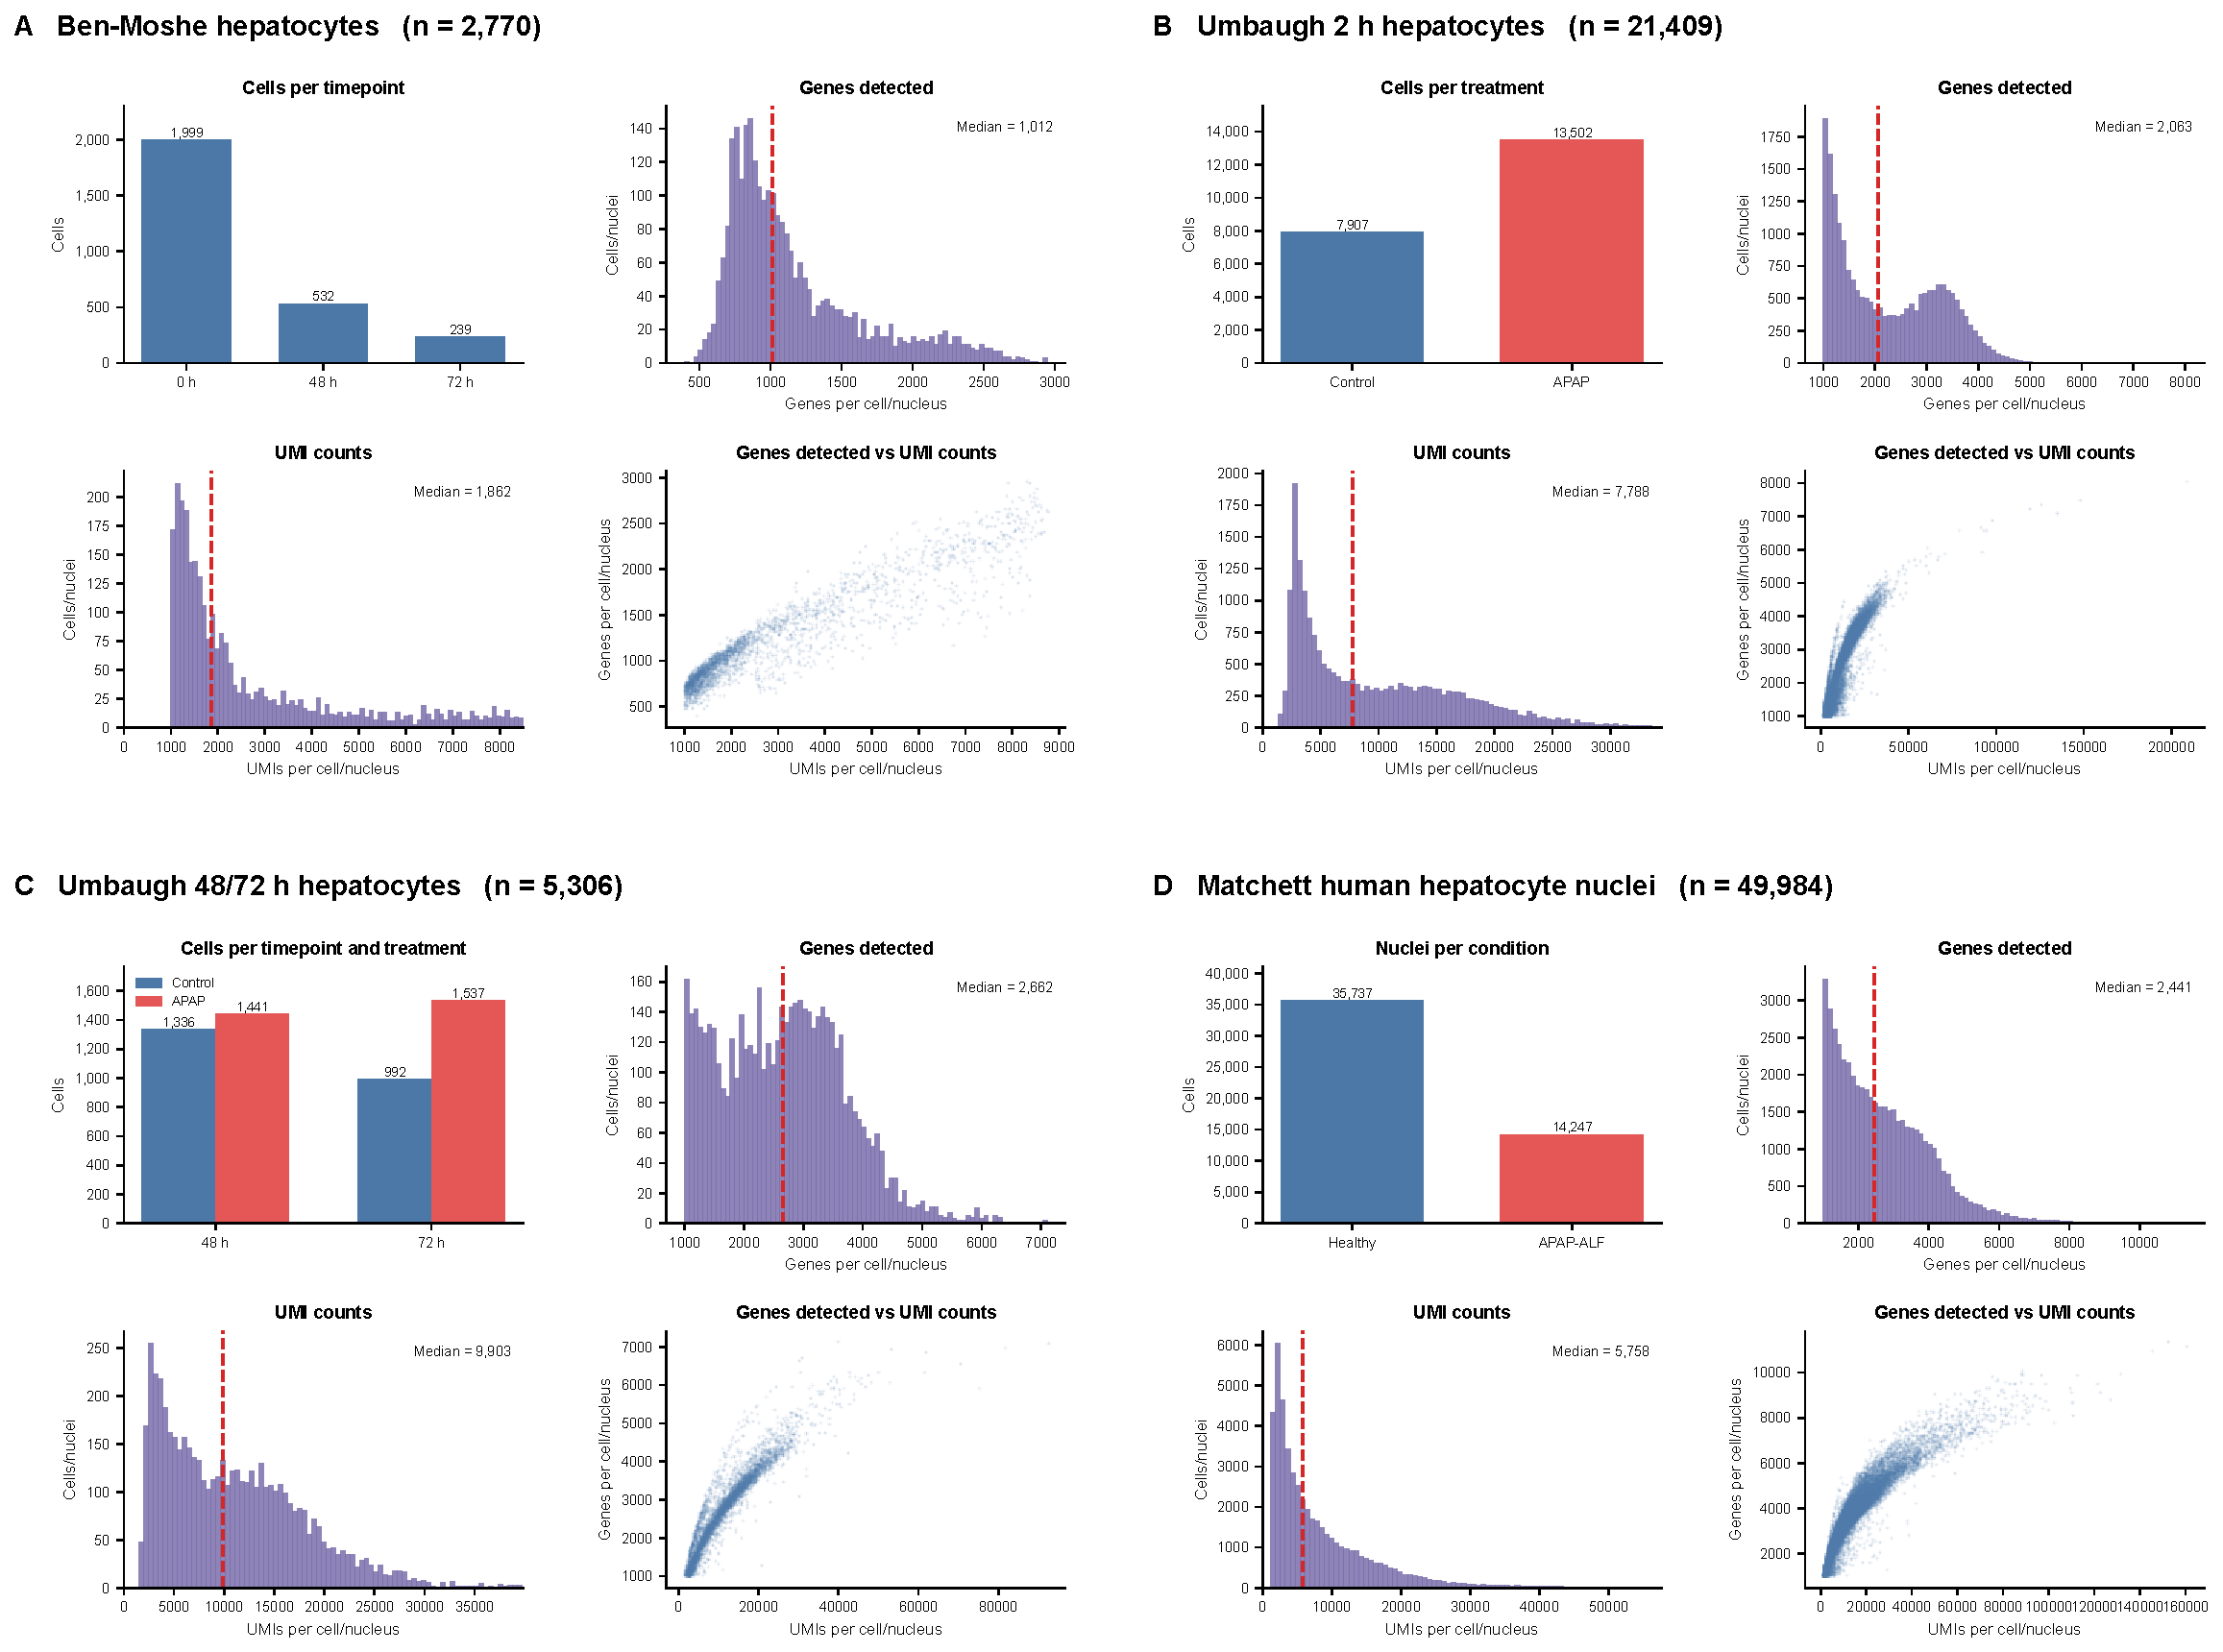
\includegraphics[width=\textwidth,trim={0.000bp 414.430bp 557.867bp 0.000bp},clip]{figures/figure_S1.pdf}
\caption{\textbf{\FigSOneTitle{}} \textbf{(A)} \FigSOneA{} \FigSOneNotes{}}
\label{fig:S1}
\end{figure}

\clearpage
\begin{figure}[H]
\centering
\ContinuedFloat
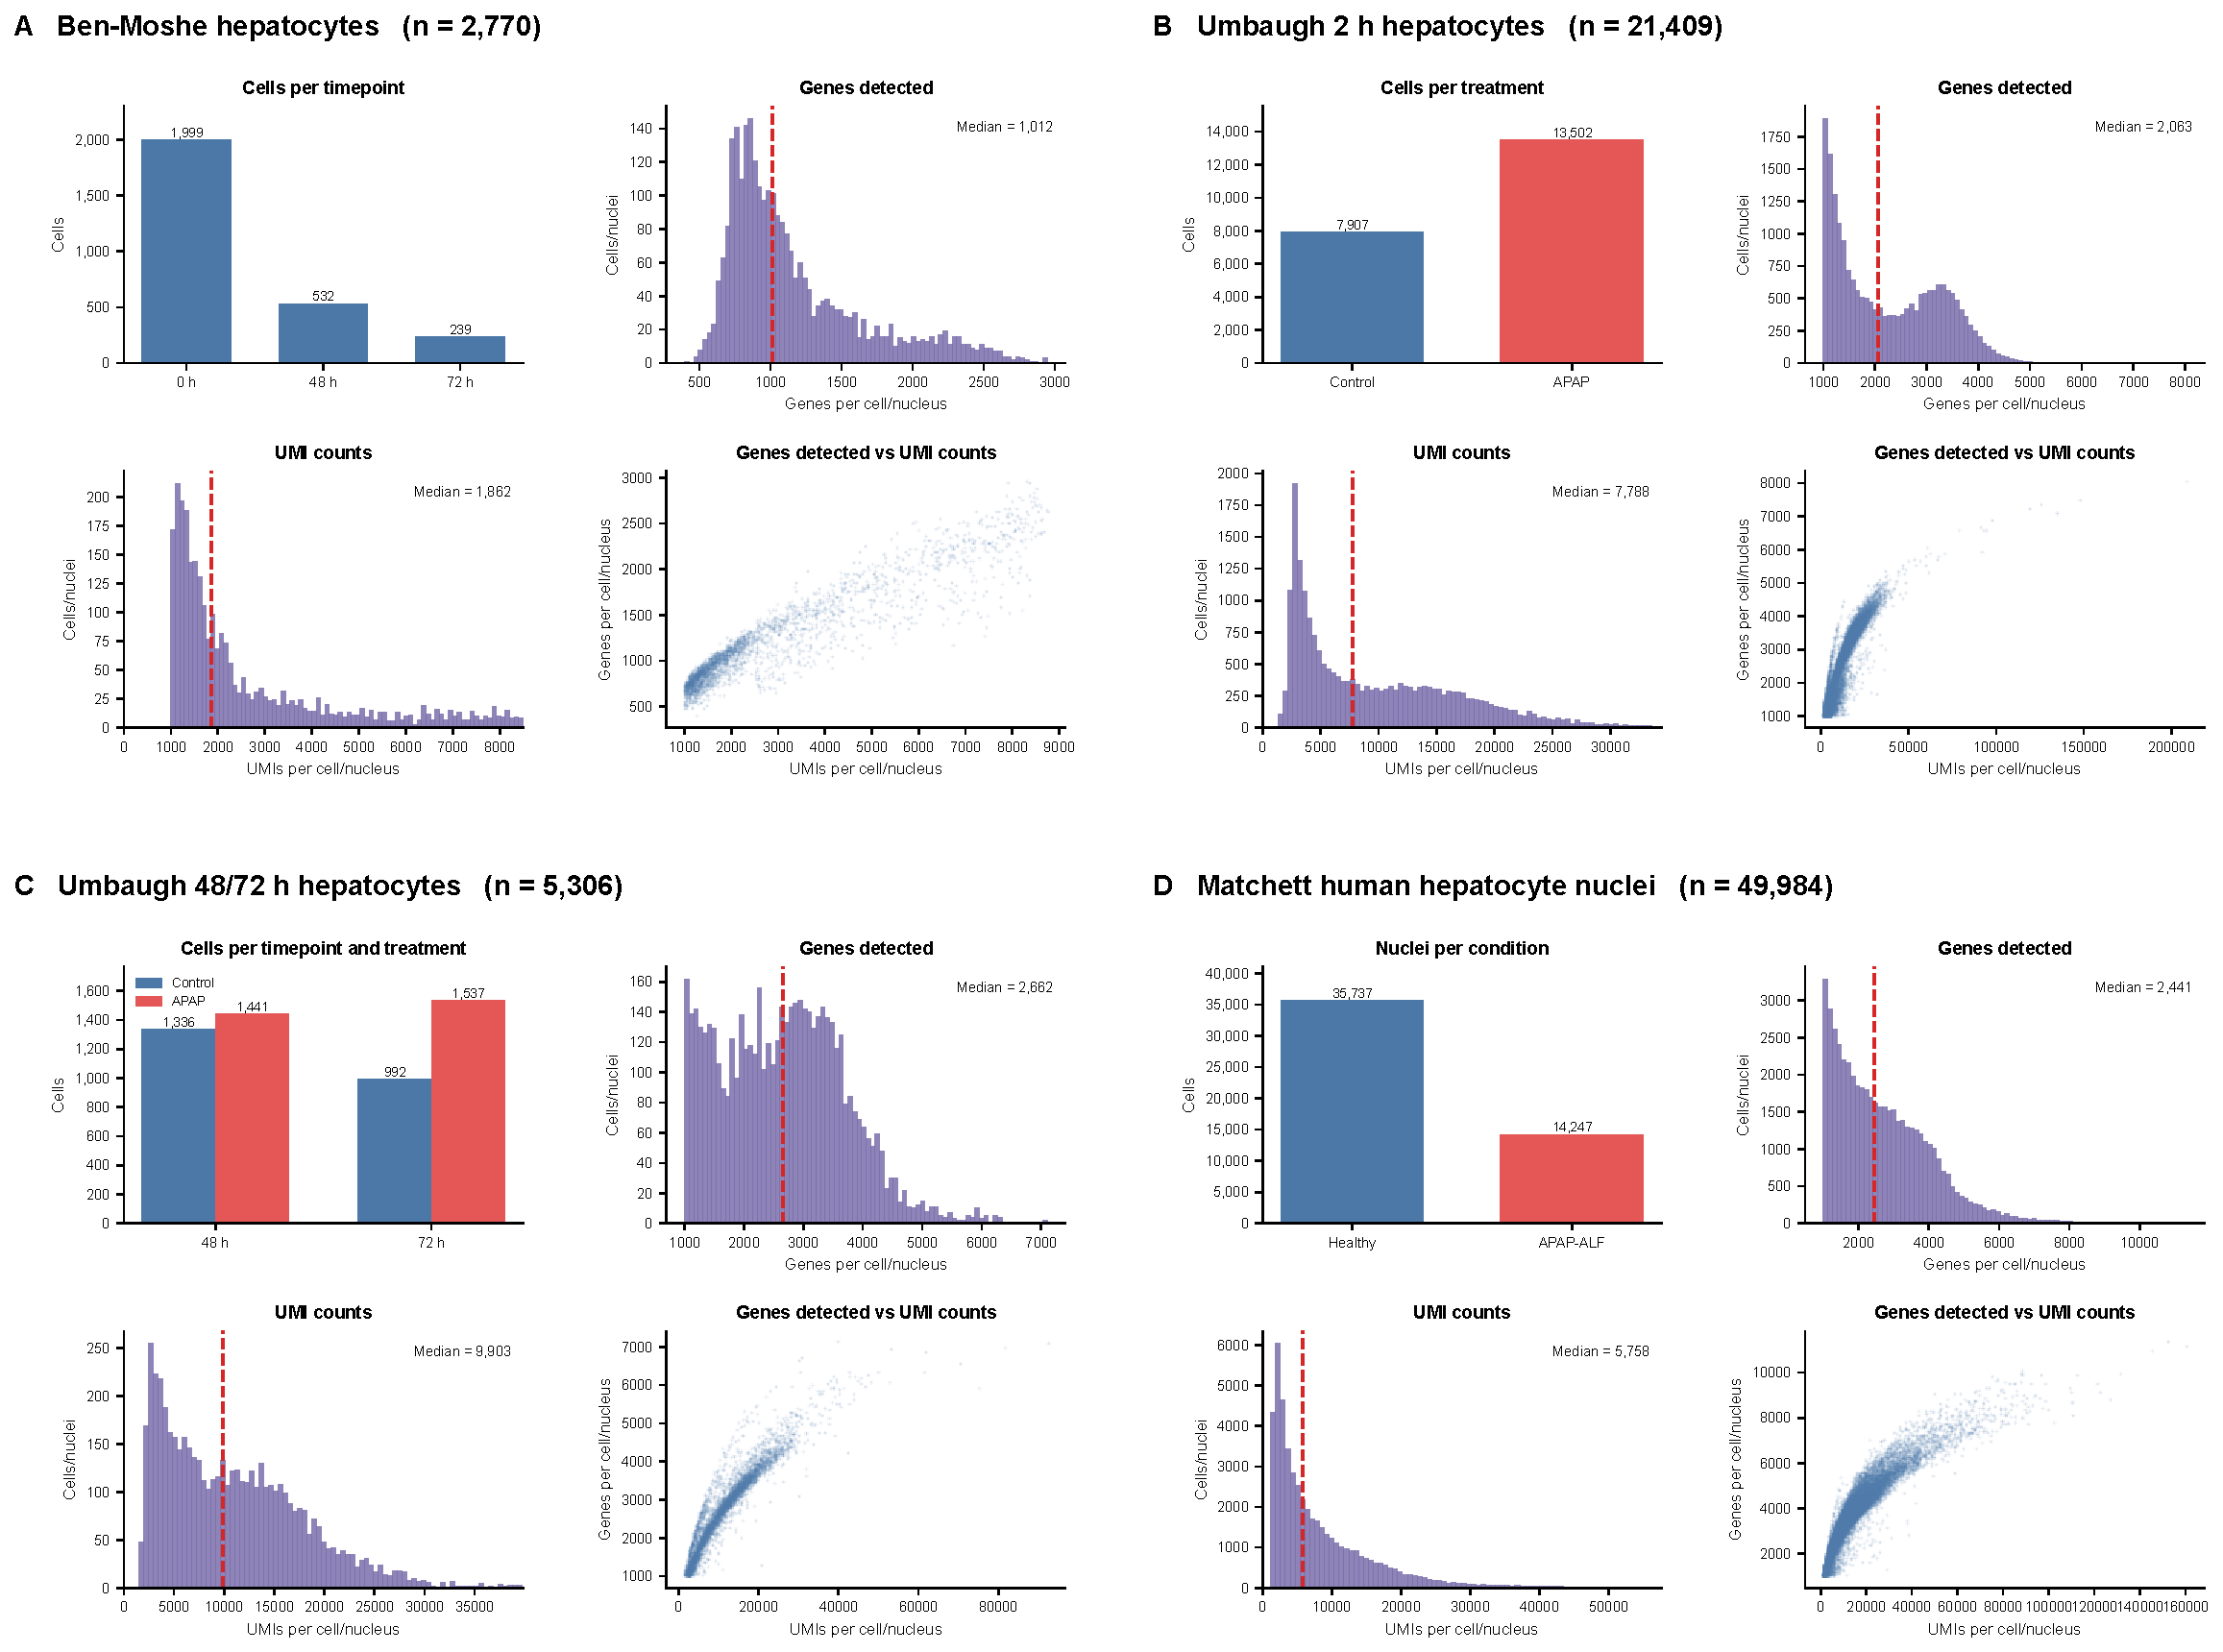
\includegraphics[width=\textwidth,trim={557.000bp 414.430bp 0.000bp 0.000bp},clip]{figures/figure_S1.pdf}
\caption{\textbf{\FigSOneTitle{} (continued)} \textbf{(B)} \FigSOneB{}}
\end{figure}

\clearpage
\begin{figure}[H]
\centering
\ContinuedFloat
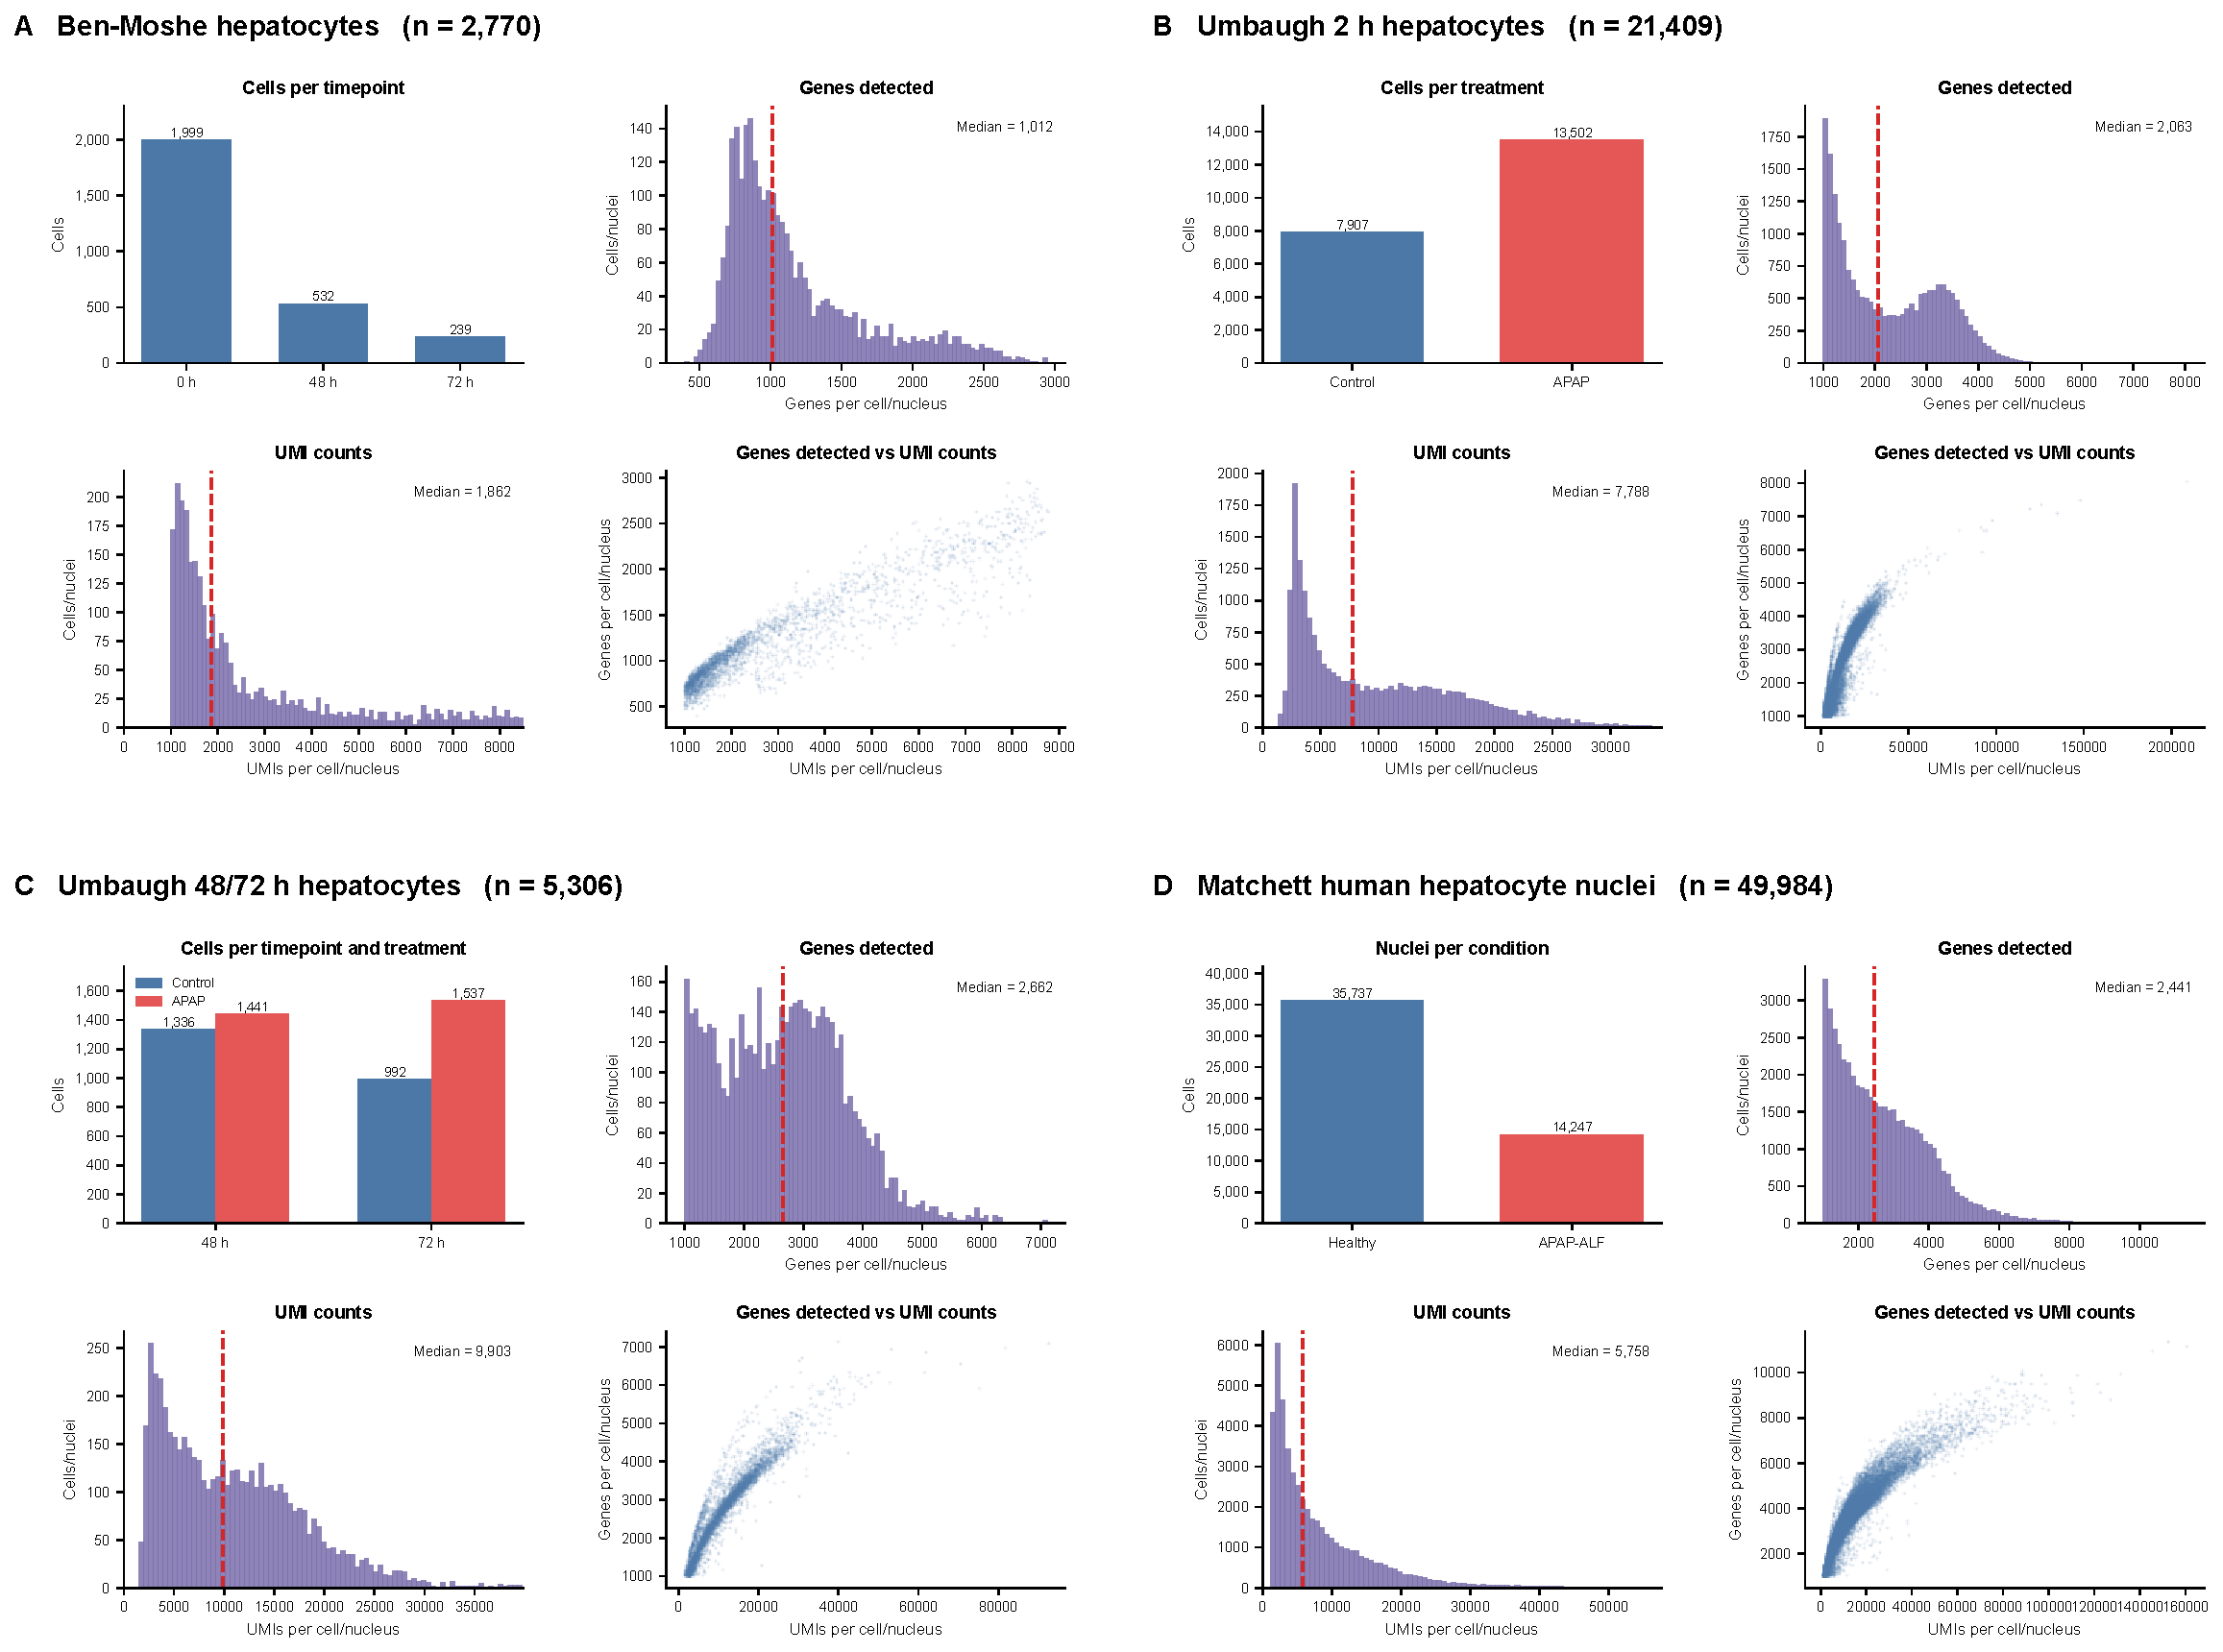
\includegraphics[width=\textwidth,trim={0.000bp 0.000bp 557.867bp 414.000bp},clip]{figures/figure_S1.pdf}
\caption{\textbf{\FigSOneTitle{} (continued)} \textbf{(C)} \FigSOneC{}}
\end{figure}

\clearpage
\begin{figure}[H]
\centering
\ContinuedFloat
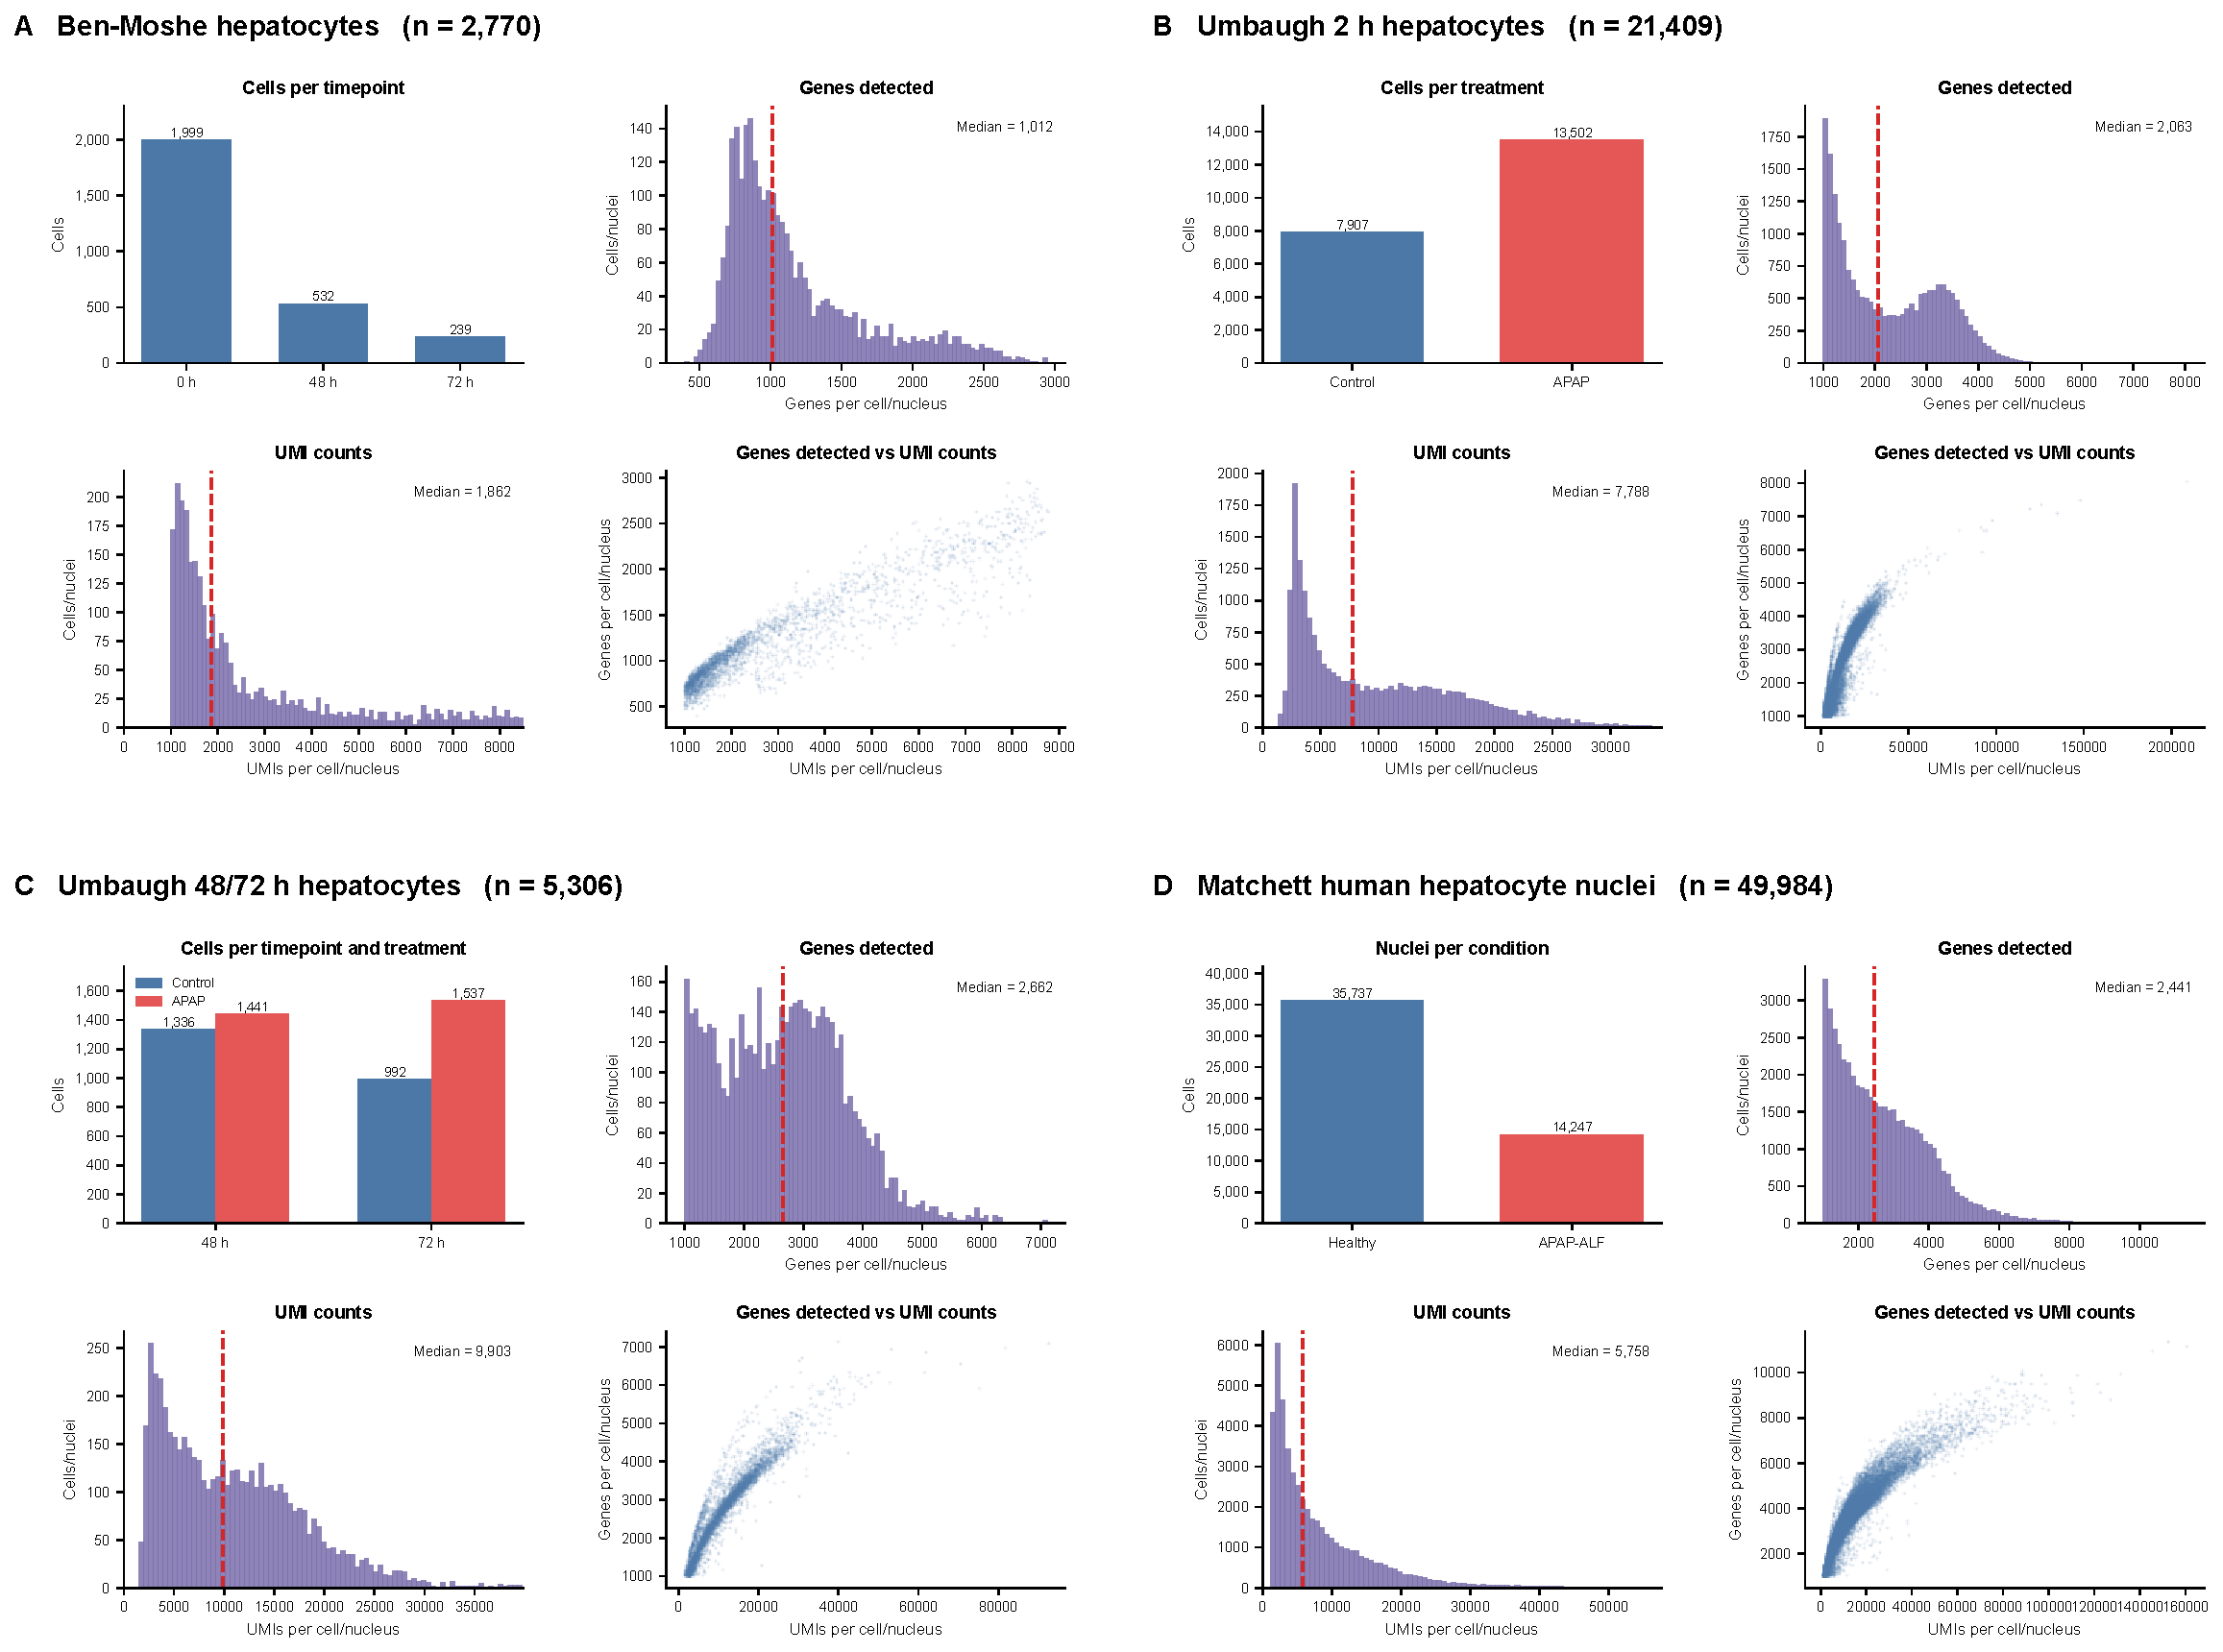
\includegraphics[width=\textwidth,trim={557.000bp 0.000bp 0.000bp 414.000bp},clip]{figures/figure_S1.pdf}
\caption{\textbf{\FigSOneTitle{} (continued)} \textbf{(D)} \FigSOneD{}}
\end{figure}

\clearpage
\begin{figure}[H]
\centering
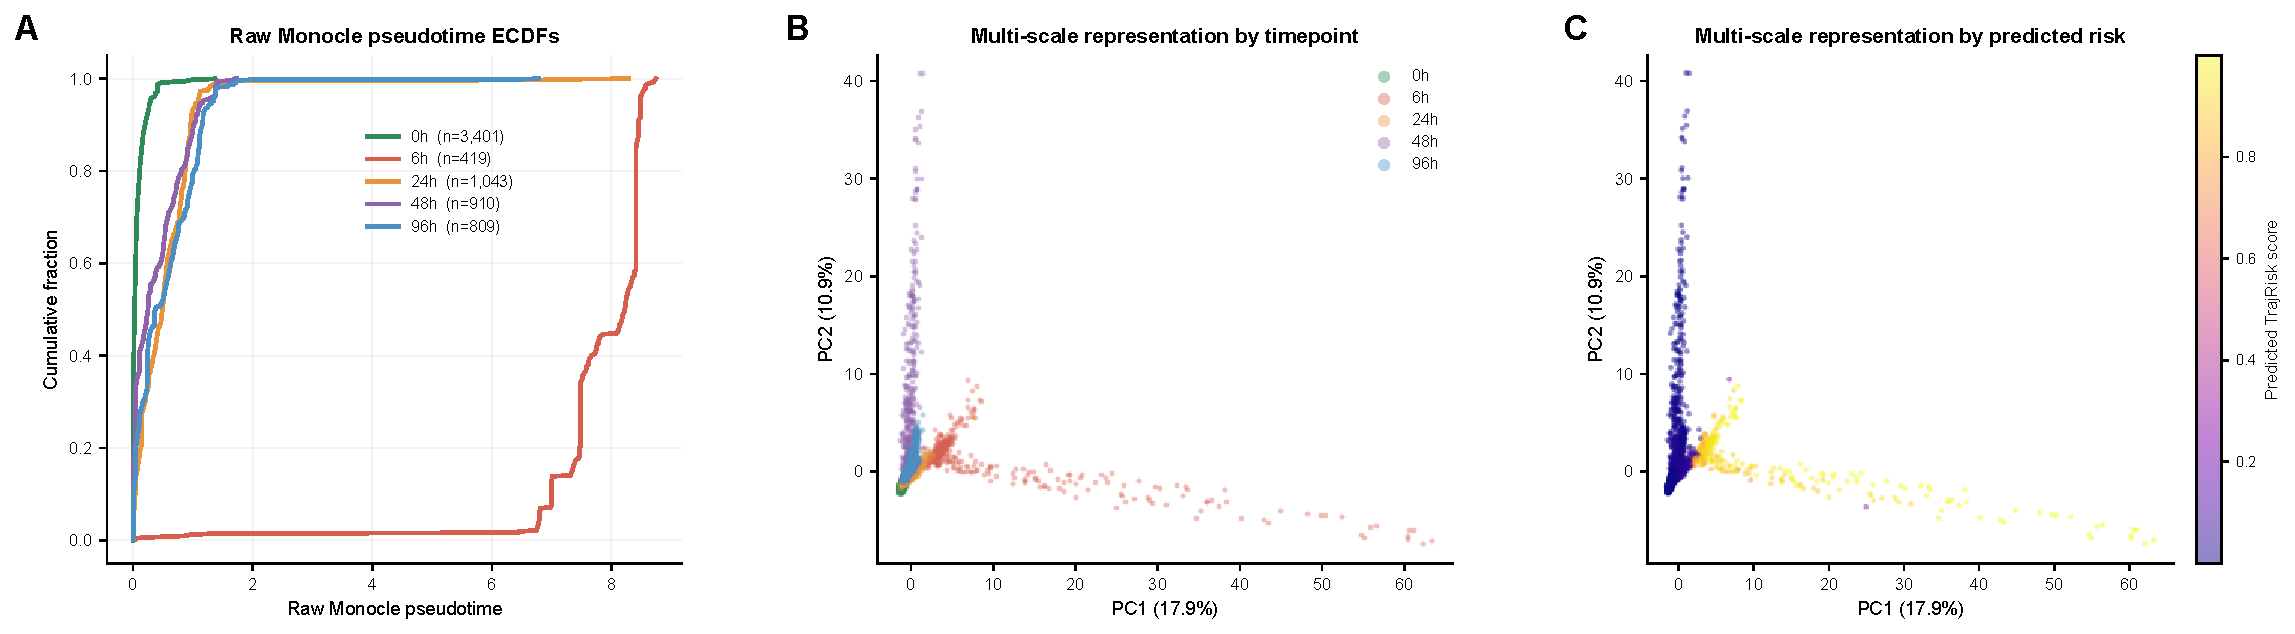
\includegraphics[width=0.78\textwidth,trim={0.000bp 0.000bp 734.759bp 0.000bp},clip]{figures/figure_S2.pdf}
\caption{\textbf{\FigSTwoTitle{}} \textbf{(A)} \FigSTwoA{} \FigSTwoNotes{}}
\label{fig:S2}
\end{figure}

\clearpage
\begin{figure}[H]
\centering
\ContinuedFloat
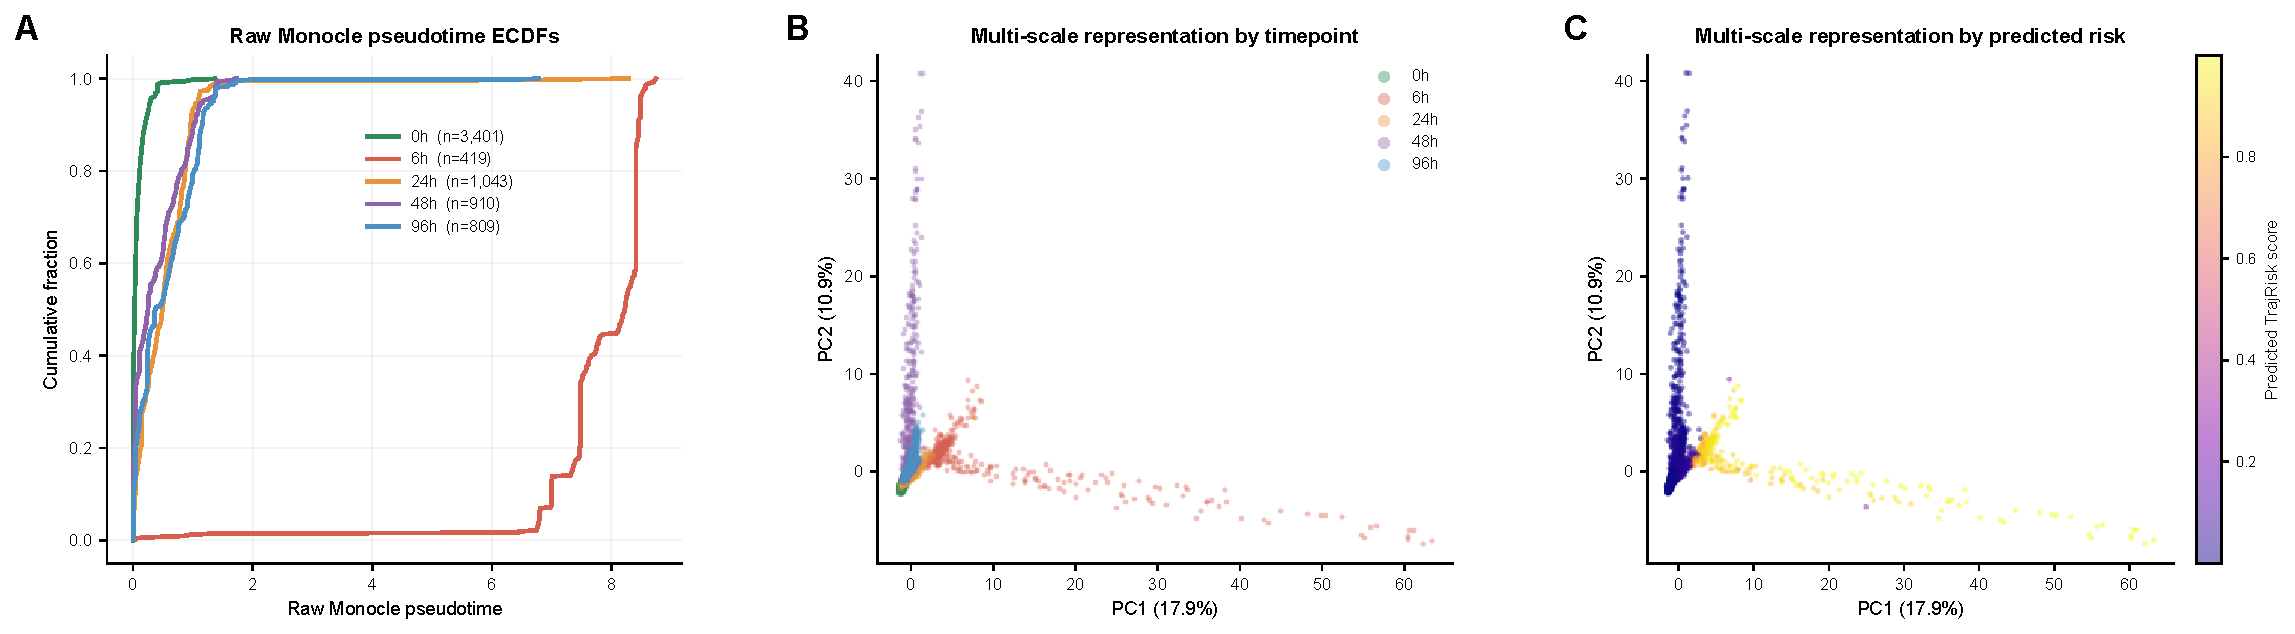
\includegraphics[width=0.64\textwidth,trim={369.000bp 0.000bp 366.759bp 0.000bp},clip]{figures/figure_S2.pdf}
\par\vspace{12pt}
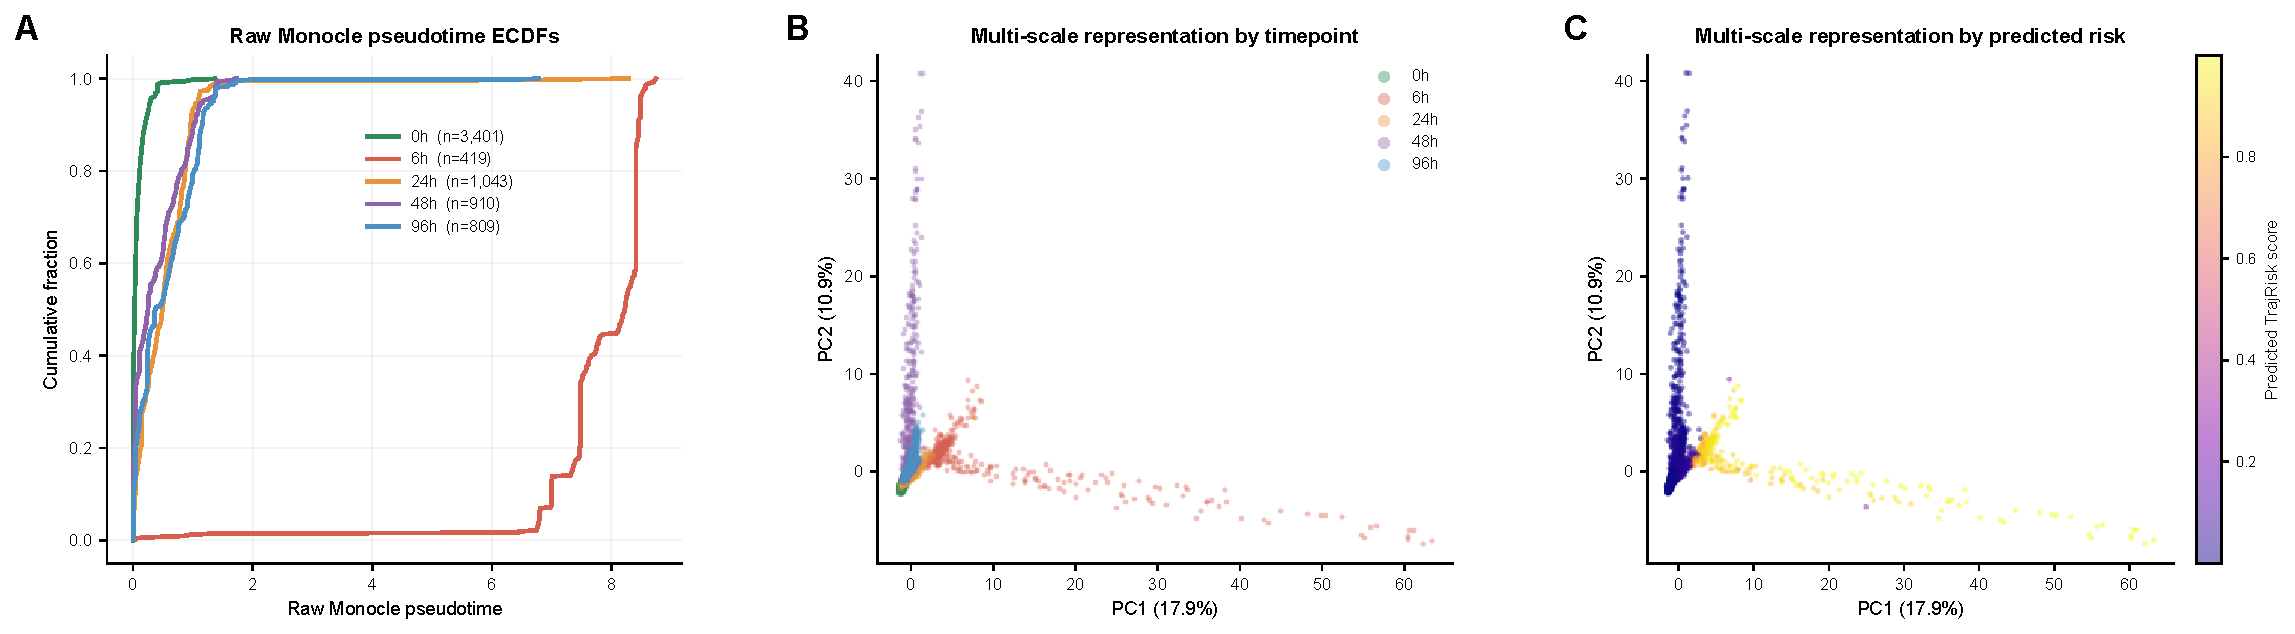
\includegraphics[width=0.64\textwidth,trim={737.000bp 0.000bp 0.000bp 0.000bp},clip]{figures/figure_S2.pdf}
\caption{\textbf{\FigSTwoTitle{} (continued)} \textbf{(B)} \FigSTwoB{} \textbf{(C)} \FigSTwoC{}}
\end{figure}

\clearpage
\begin{figure}[H]
\centering
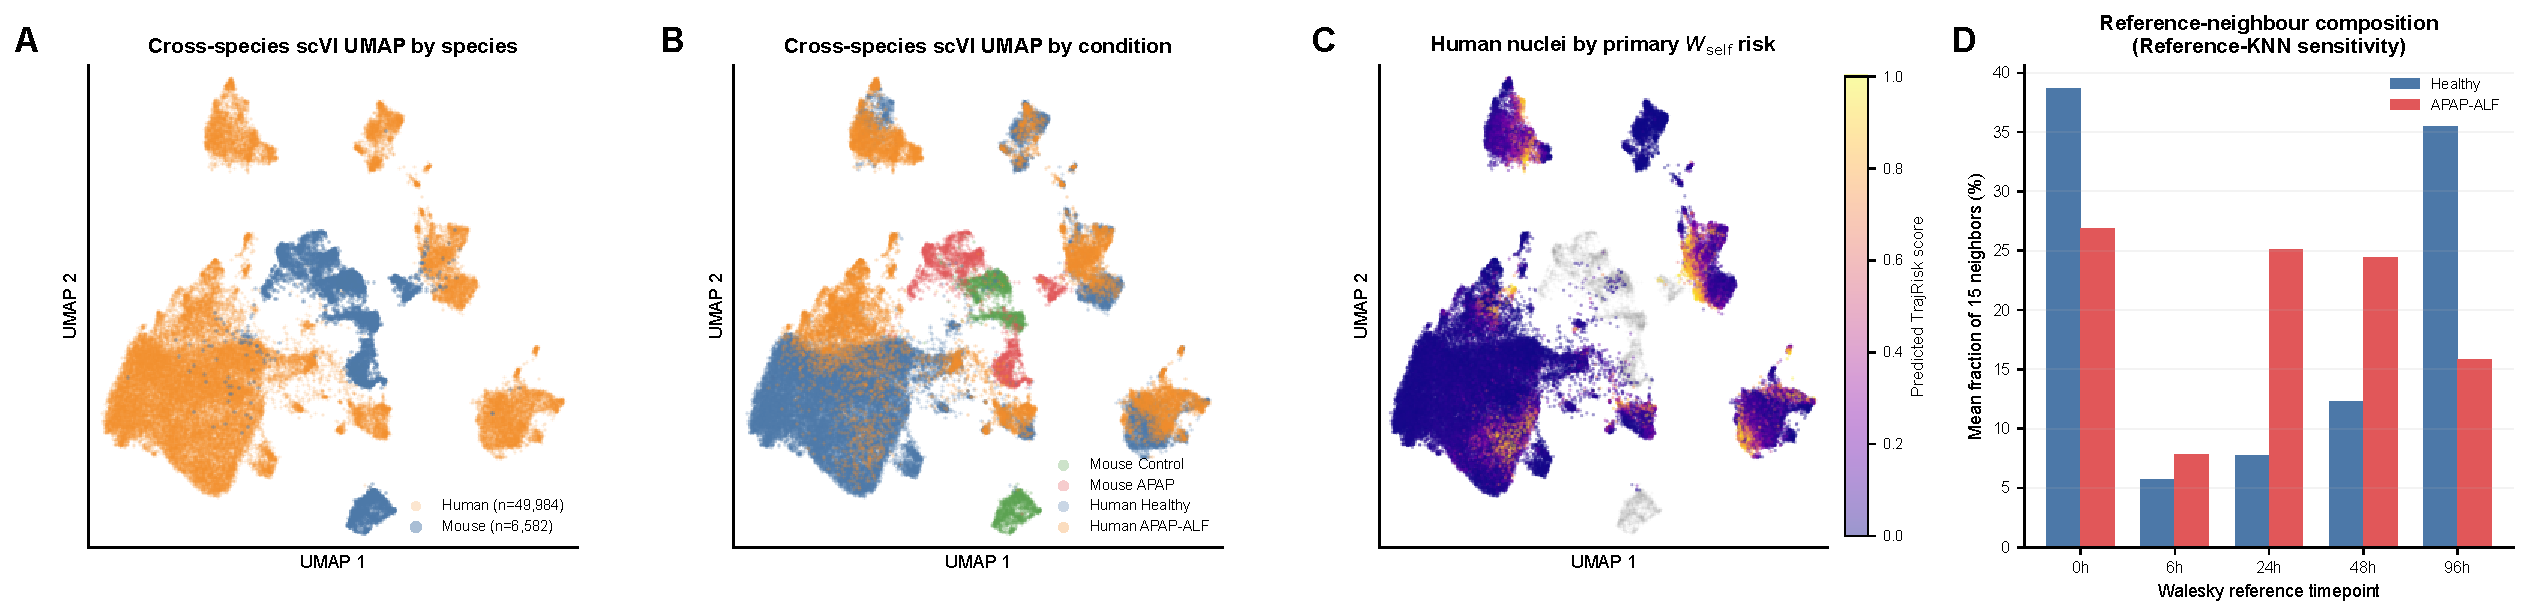
\includegraphics[width=0.492\textwidth,trim={0.000bp 0.000bp 911.701bp 0.000bp},clip]{figures/figure_S3.pdf}\hfill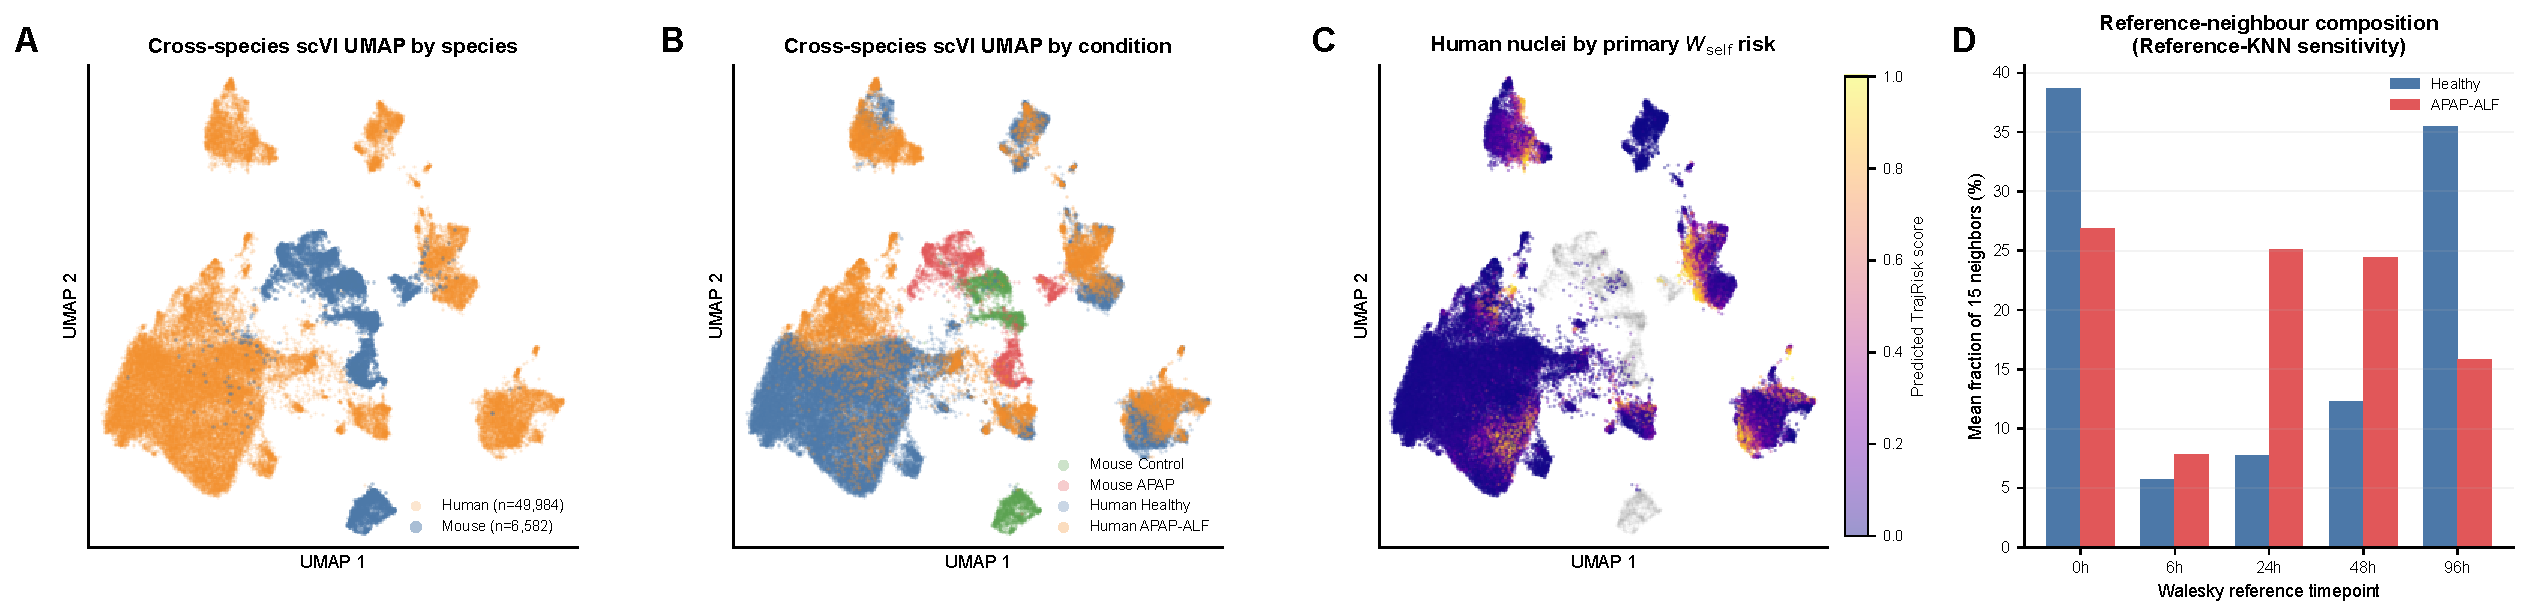
\includegraphics[width=0.492\textwidth,trim={303.000bp 0.000bp 607.701bp 0.000bp},clip]{figures/figure_S3.pdf}
\par\vspace{12pt}
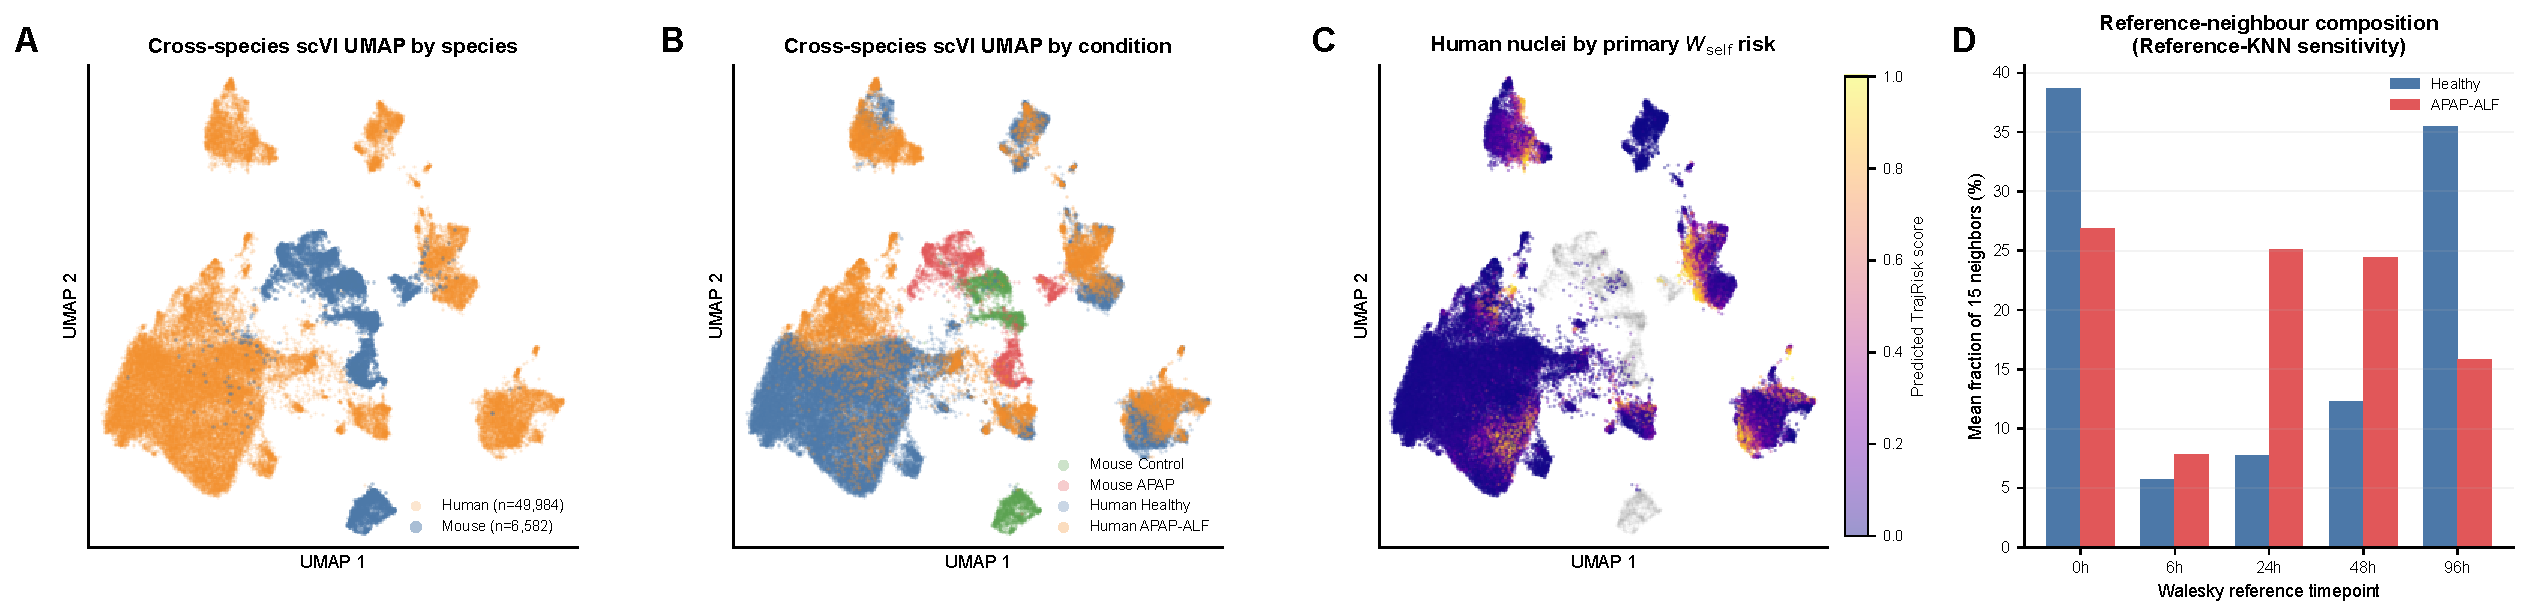
\includegraphics[width=0.526\textwidth,trim={607.000bp 0.000bp 283.701bp 0.000bp},clip]{figures/figure_S3.pdf}\hfill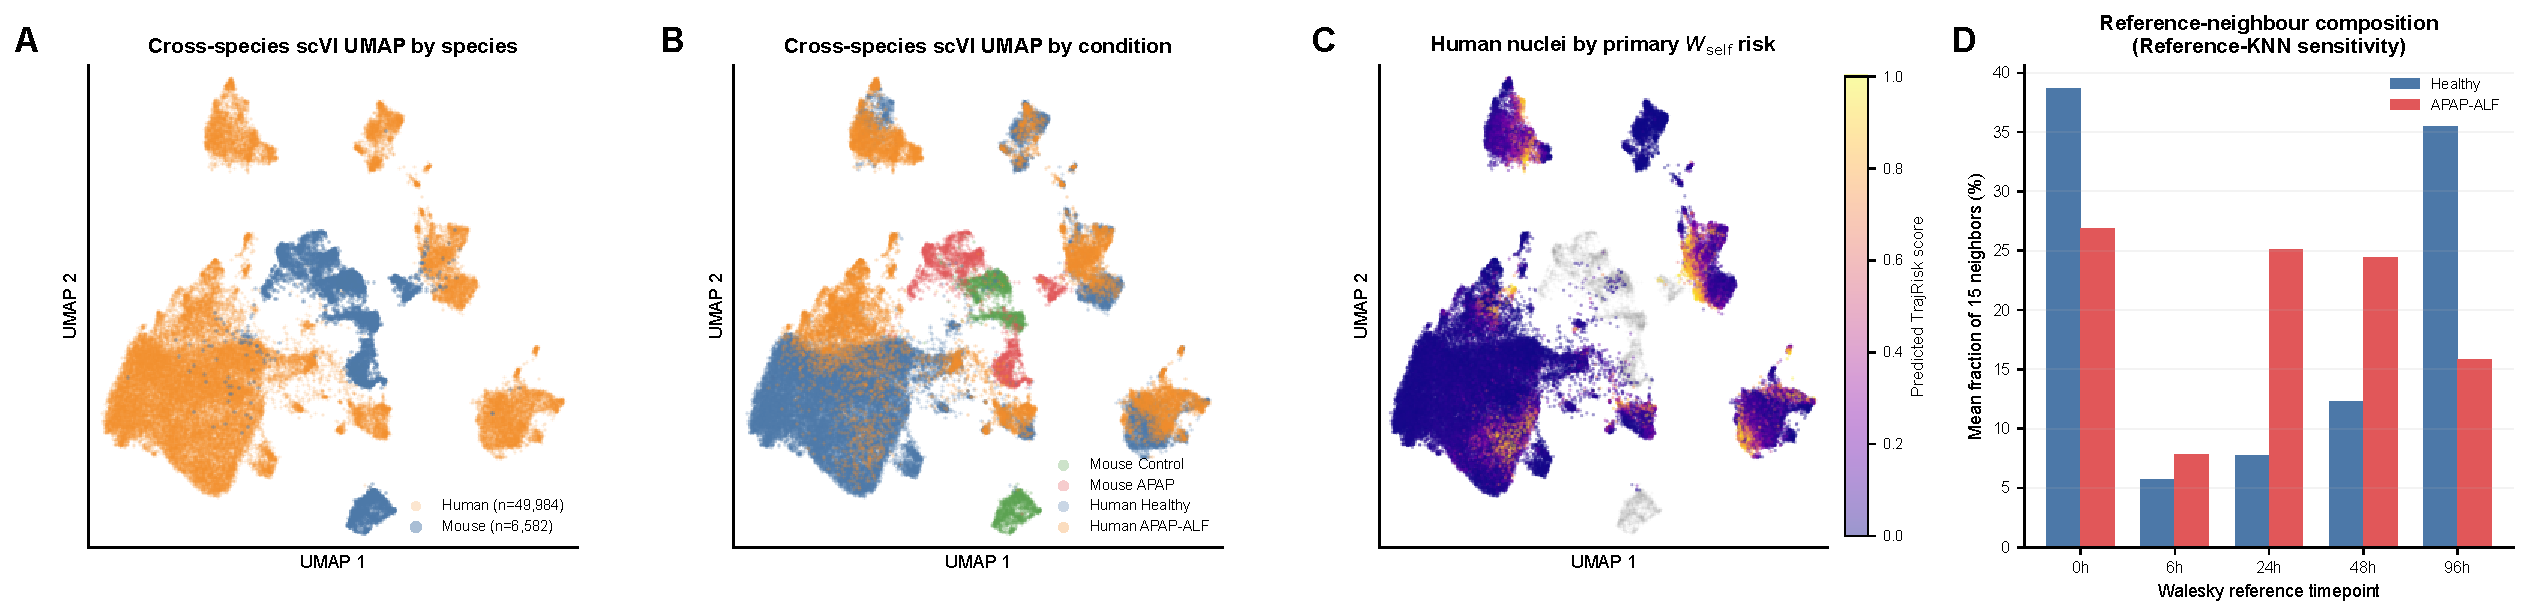
\includegraphics[width=0.460\textwidth,trim={931.000bp 0.000bp 0.000bp 0.000bp},clip]{figures/figure_S3.pdf}
\caption{\textbf{\FigSThreeTitle{}} \textbf{(A)} \FigSThreeA{} \textbf{(B)} \FigSThreeB{} \textbf{(C)} \FigSThreeC{} \textbf{(D)} \FigSThreeD{} \FigSThreeNotes{}}
\label{fig:S3}
\end{figure}

\clearpage
\begin{figure}[H]
\centering
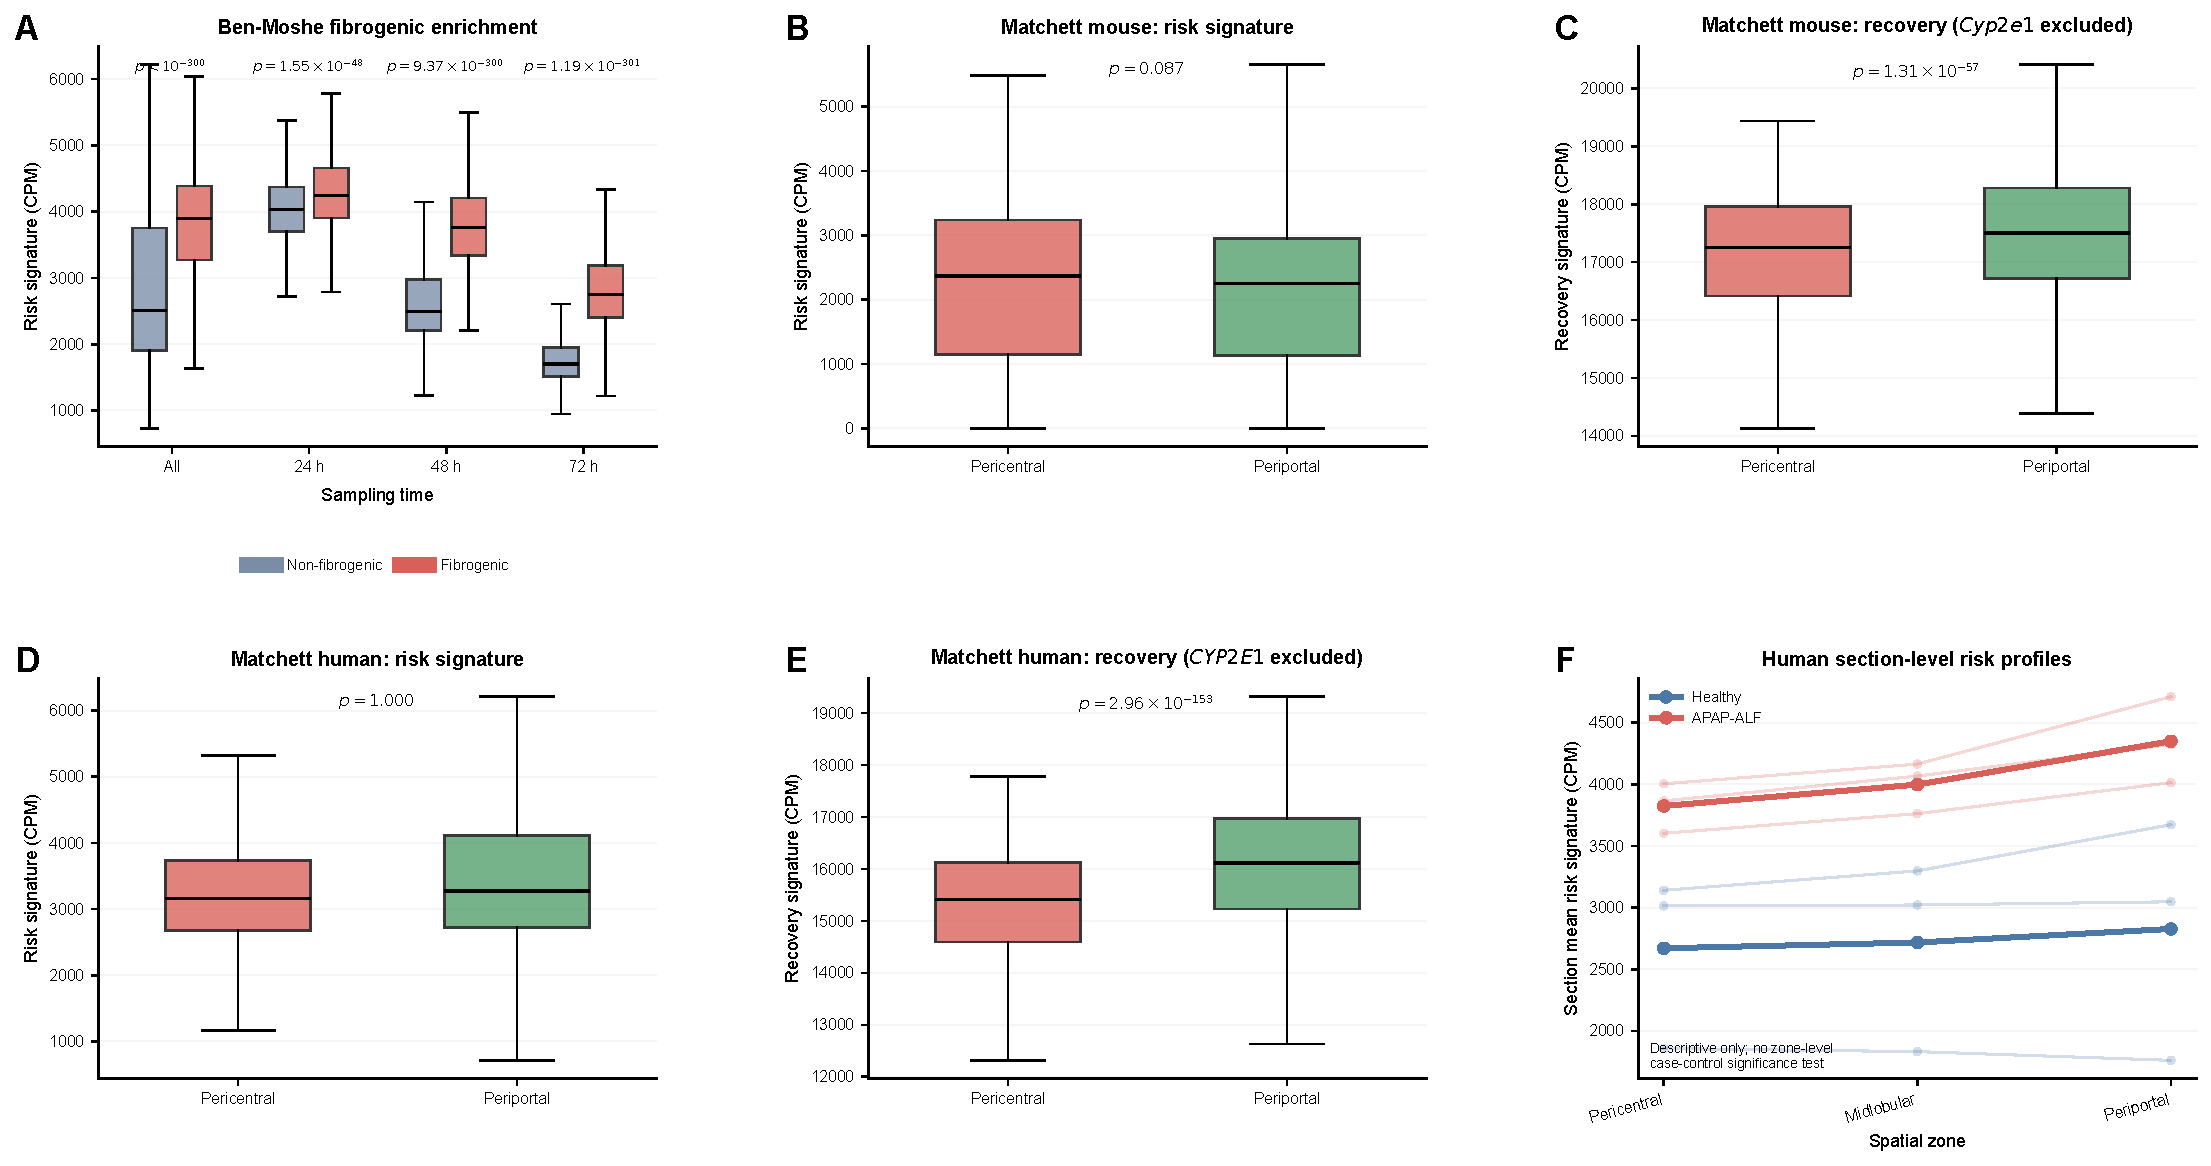
\includegraphics[width=0.74\textwidth,trim={0.000bp 286.872bp 706.415bp 0.000bp},clip]{figures/figure_S4.pdf}
\par\vspace{12pt}
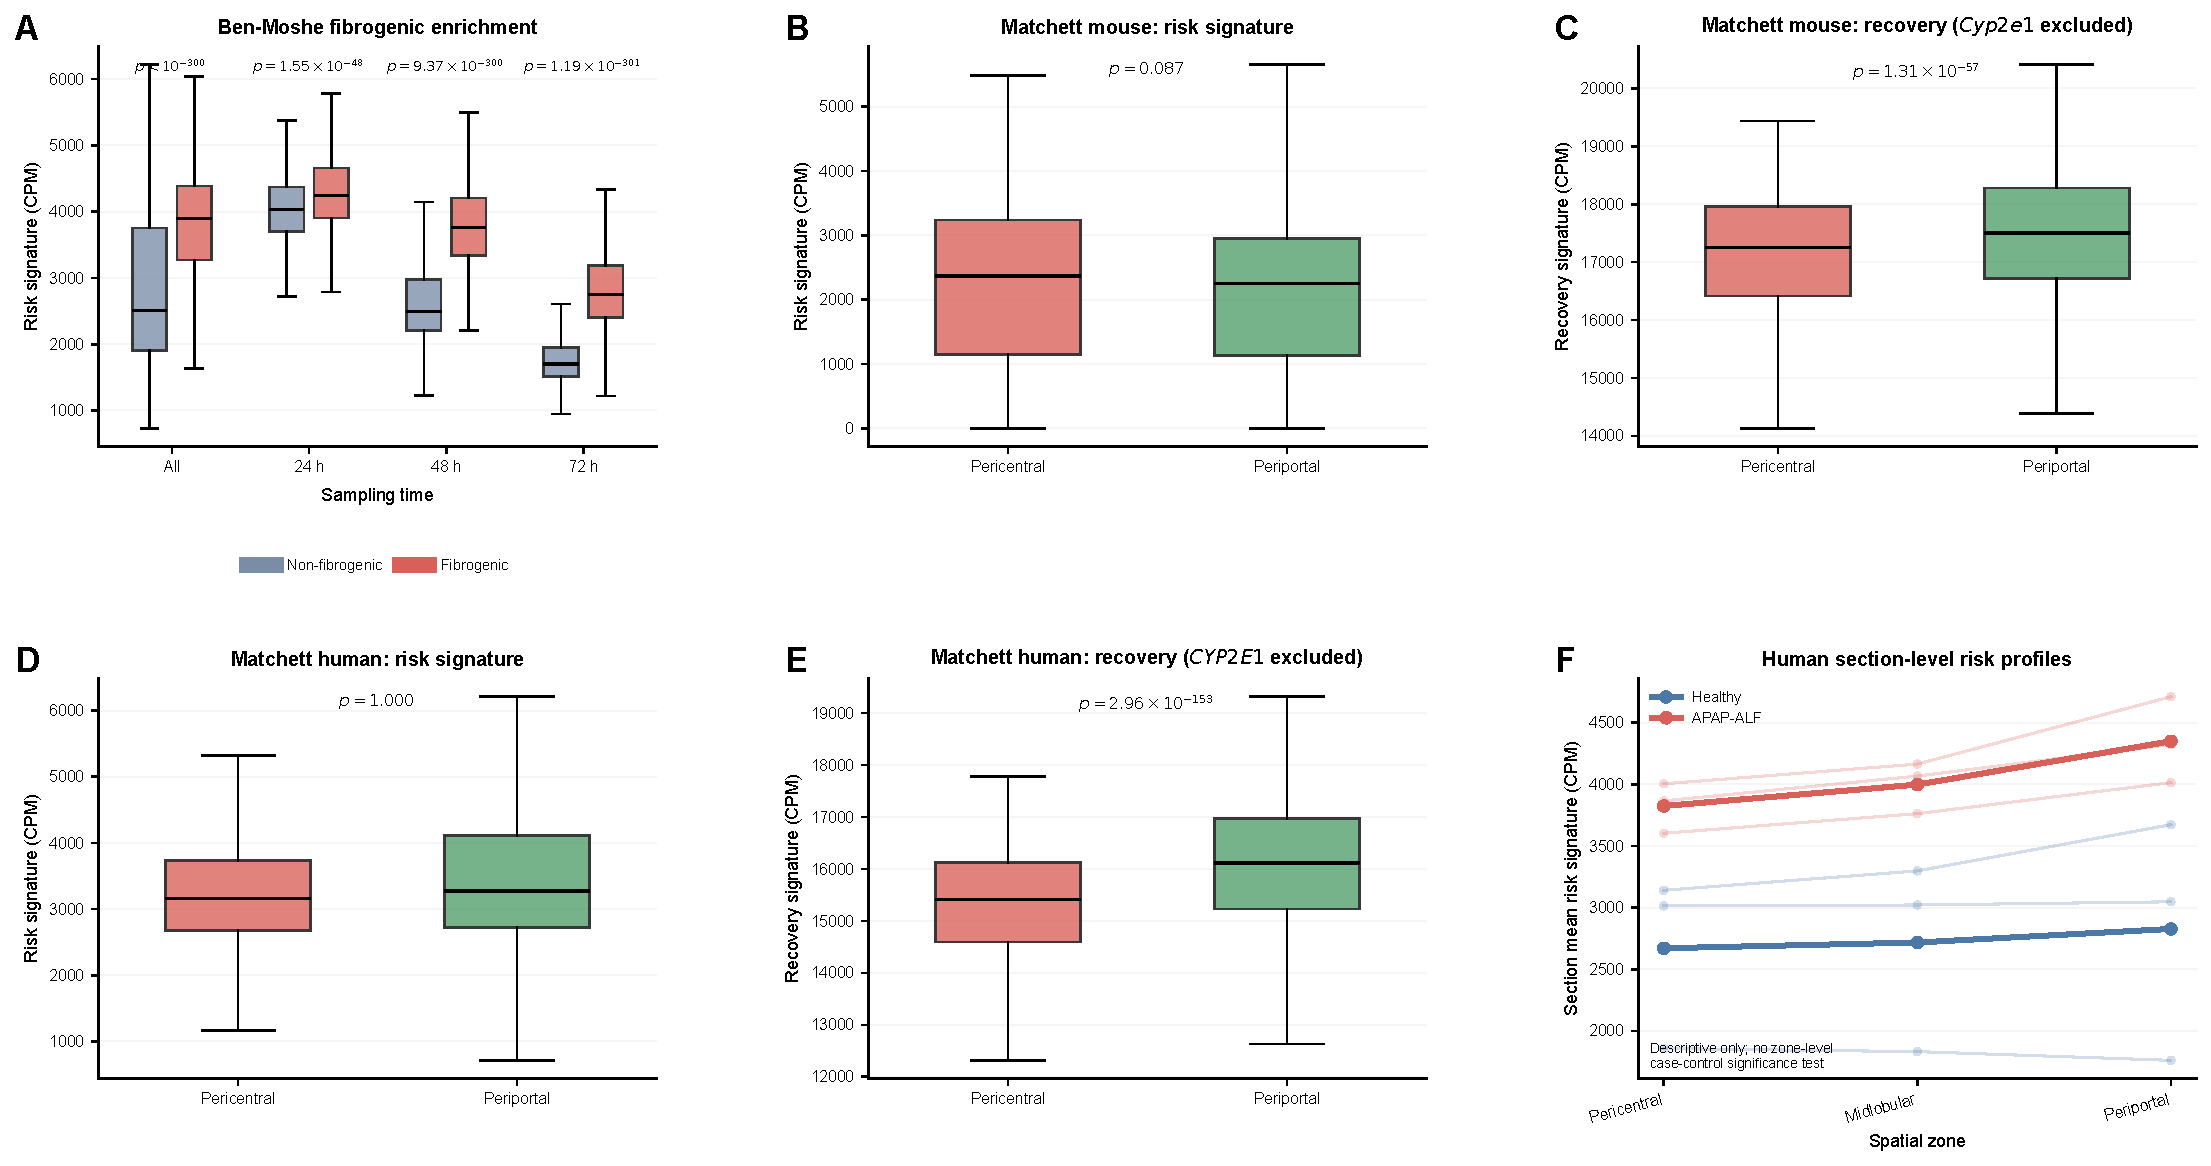
\includegraphics[width=0.64\textwidth,trim={356.000bp 286.872bp 354.415bp 0.000bp},clip]{figures/figure_S4.pdf}
\caption{\textbf{\FigSFourTitle{}} \textbf{(A)} \FigSFourA{} \textbf{(B)} \FigSFourB{}}
\label{fig:S4}
\end{figure}

\clearpage
\begin{figure}[H]
\centering
\ContinuedFloat
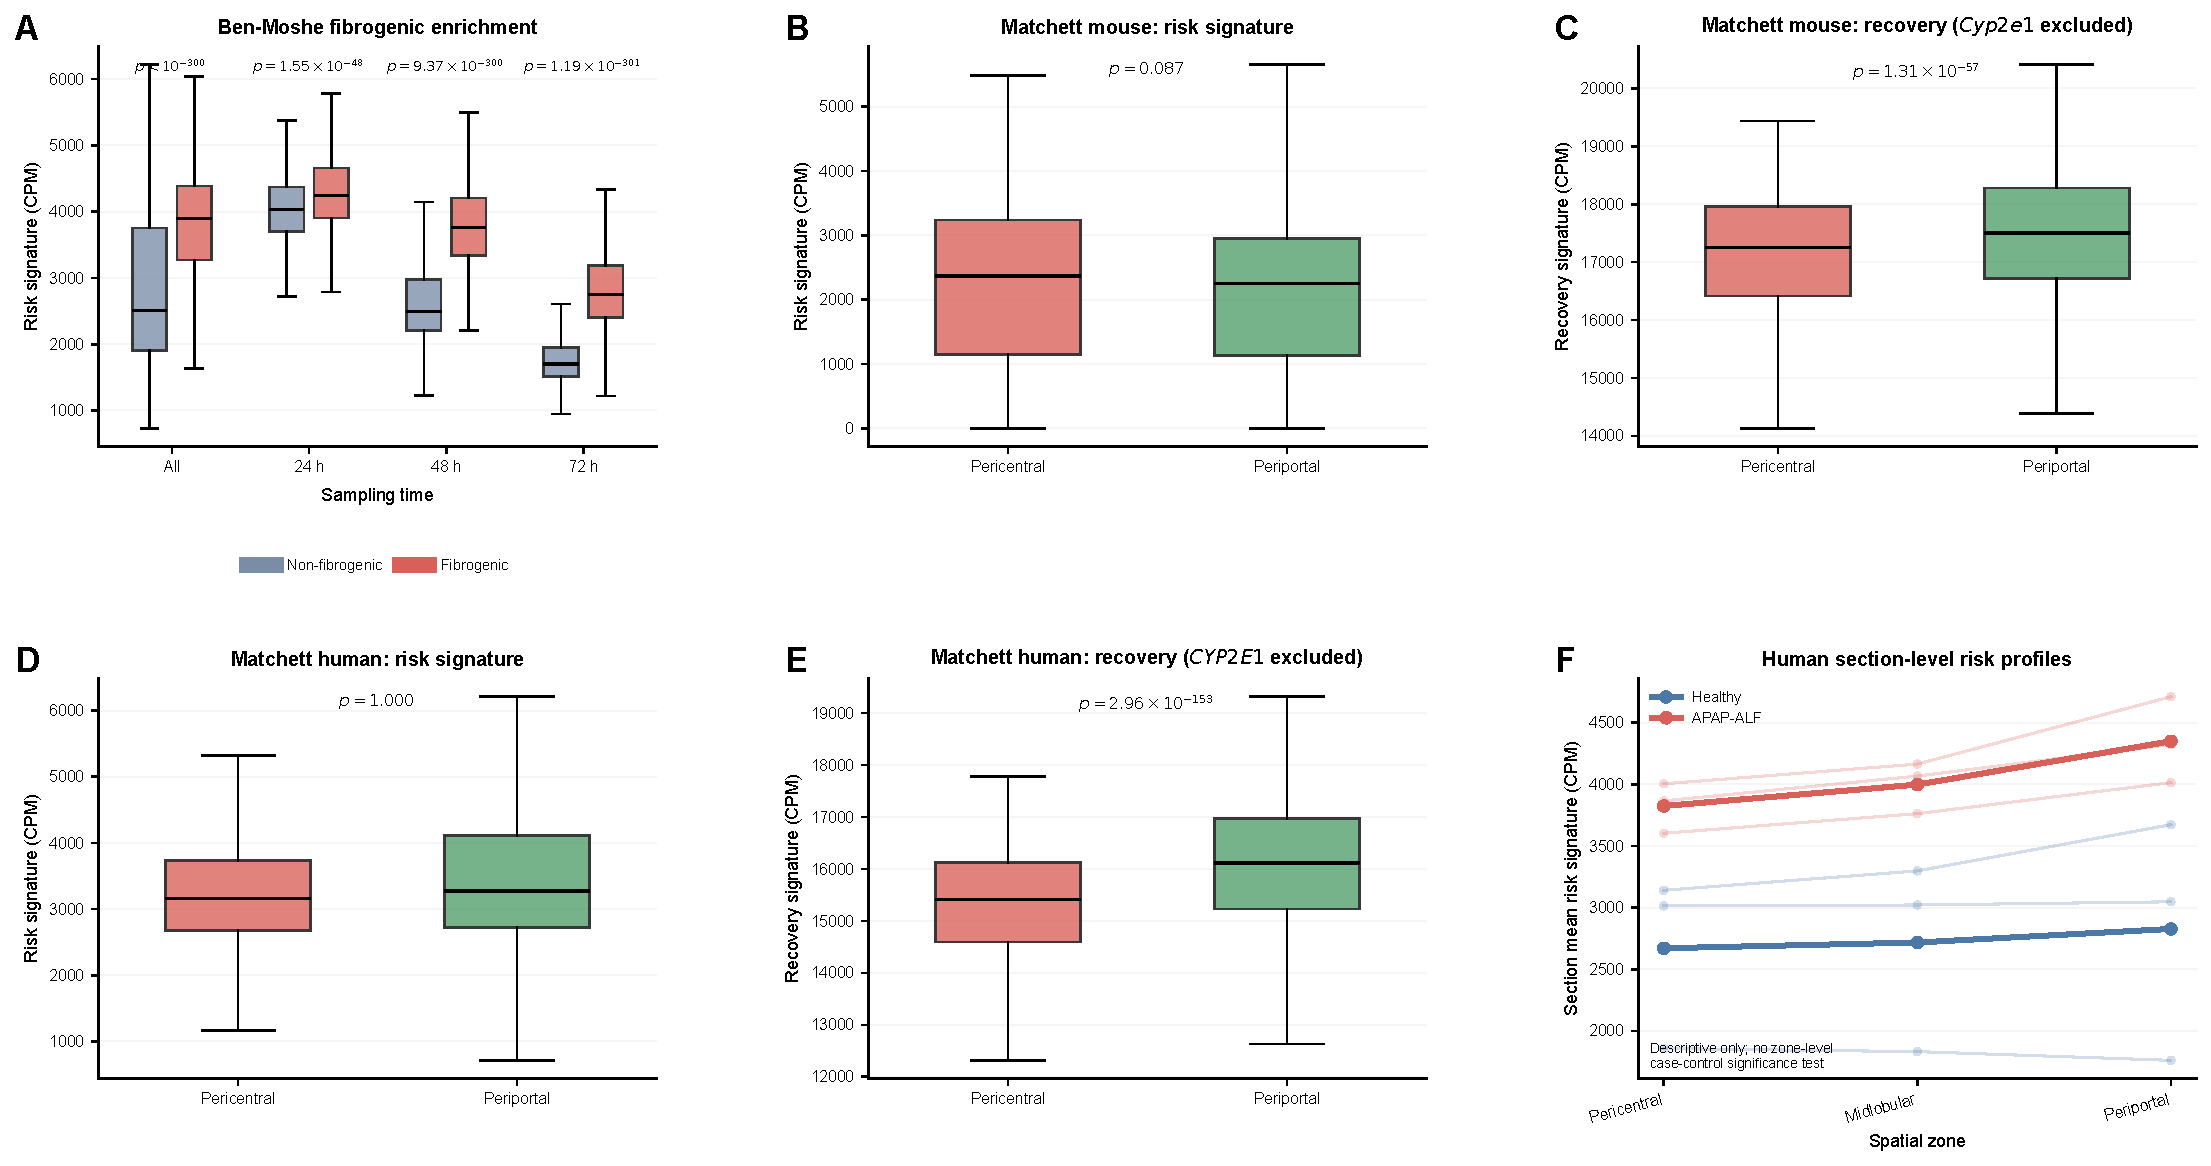
\includegraphics[width=0.64\textwidth,trim={708.000bp 286.872bp 0.000bp 0.000bp},clip]{figures/figure_S4.pdf}
\par\vspace{12pt}
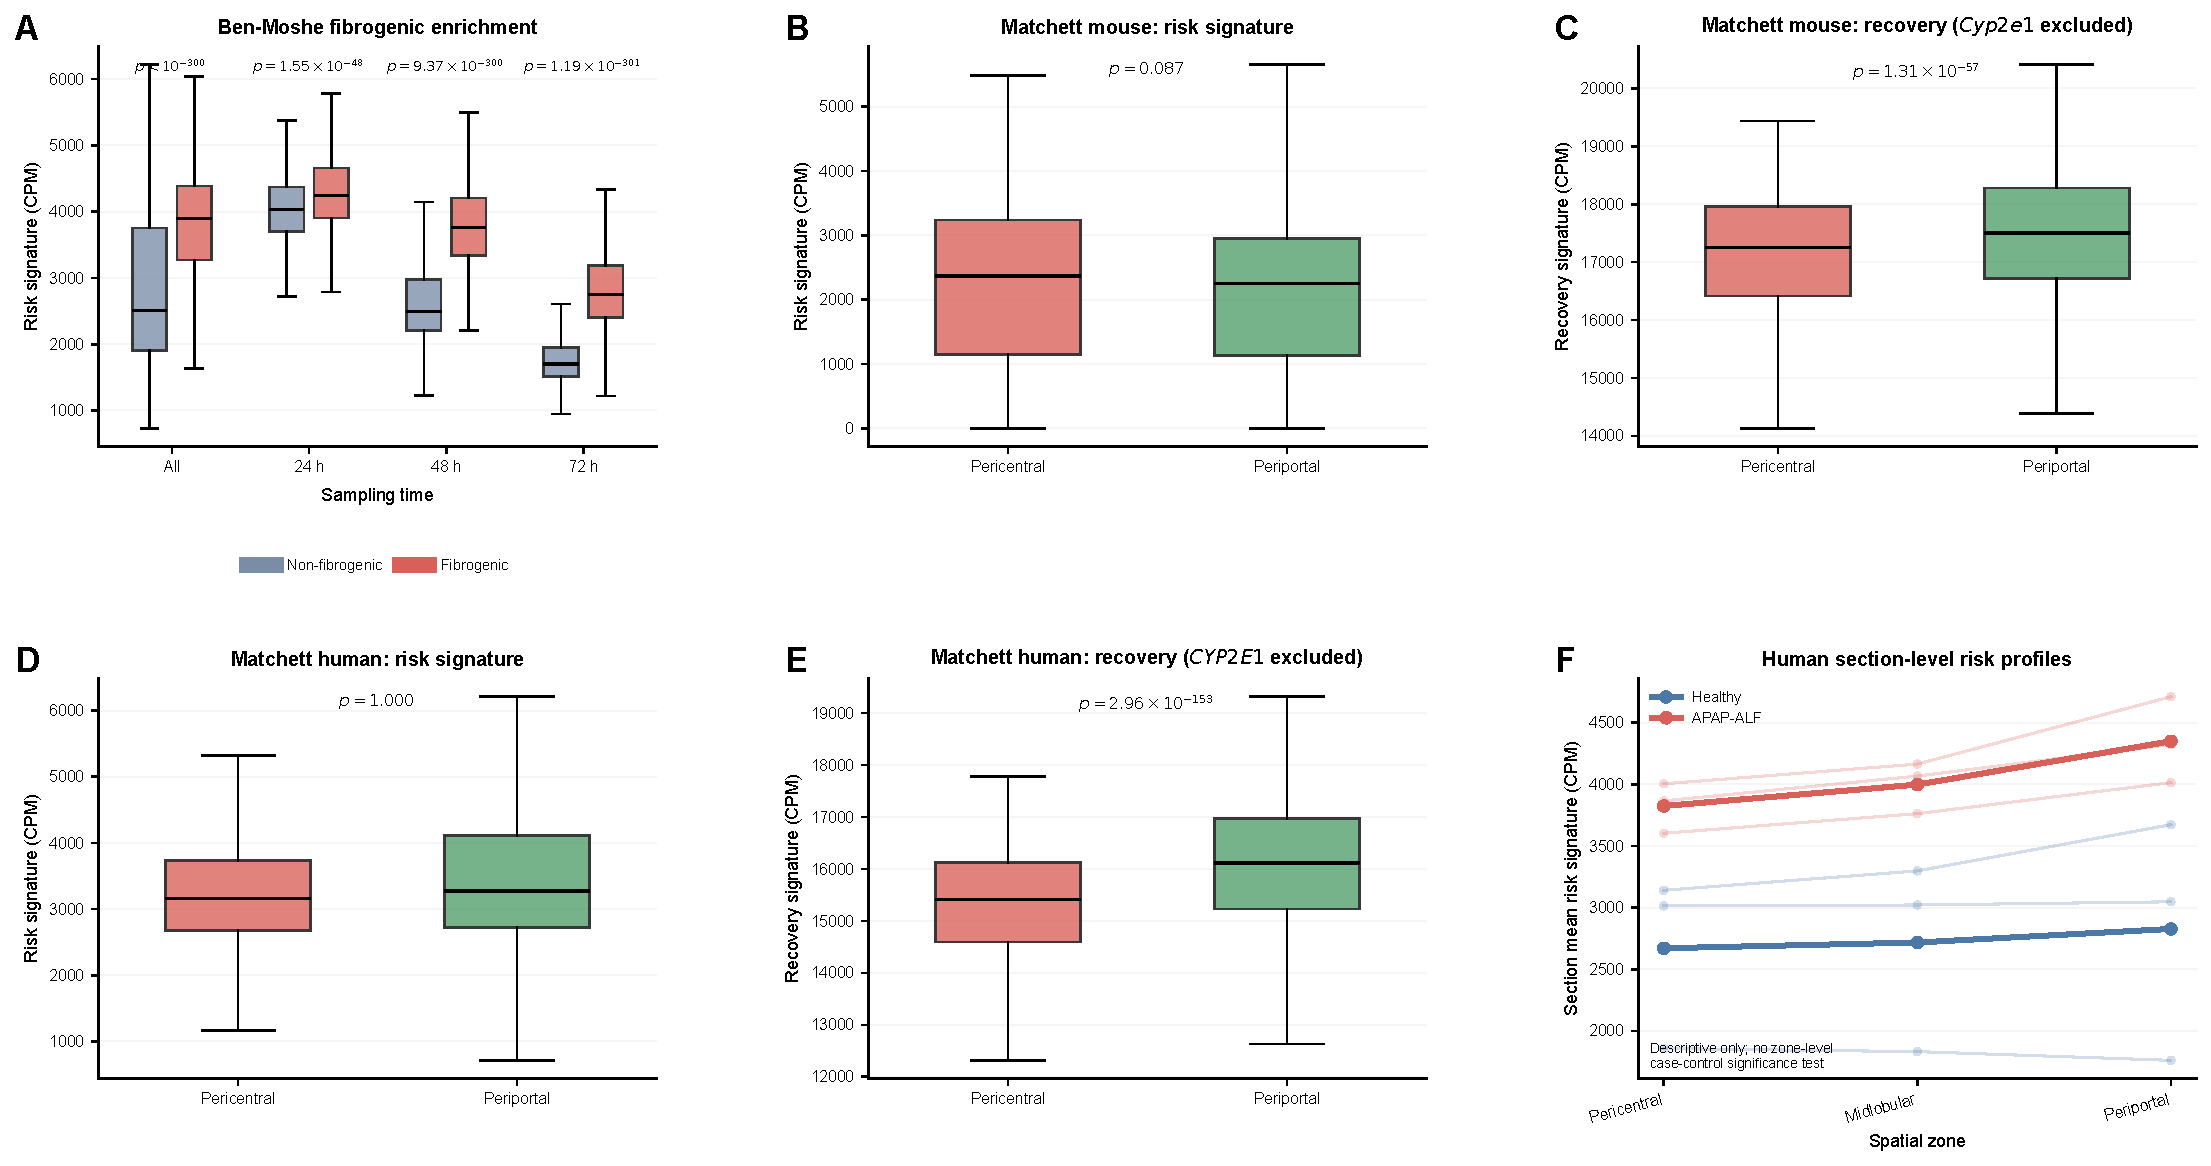
\includegraphics[width=0.64\textwidth,trim={0.000bp 0.000bp 706.415bp 285.000bp},clip]{figures/figure_S4.pdf}
\caption{\textbf{\FigSFourTitle{} (continued)} \textbf{(C)} \FigSFourC{} \textbf{(D)} \FigSFourD{}}
\end{figure}

\clearpage
\begin{figure}[H]
\centering
\ContinuedFloat
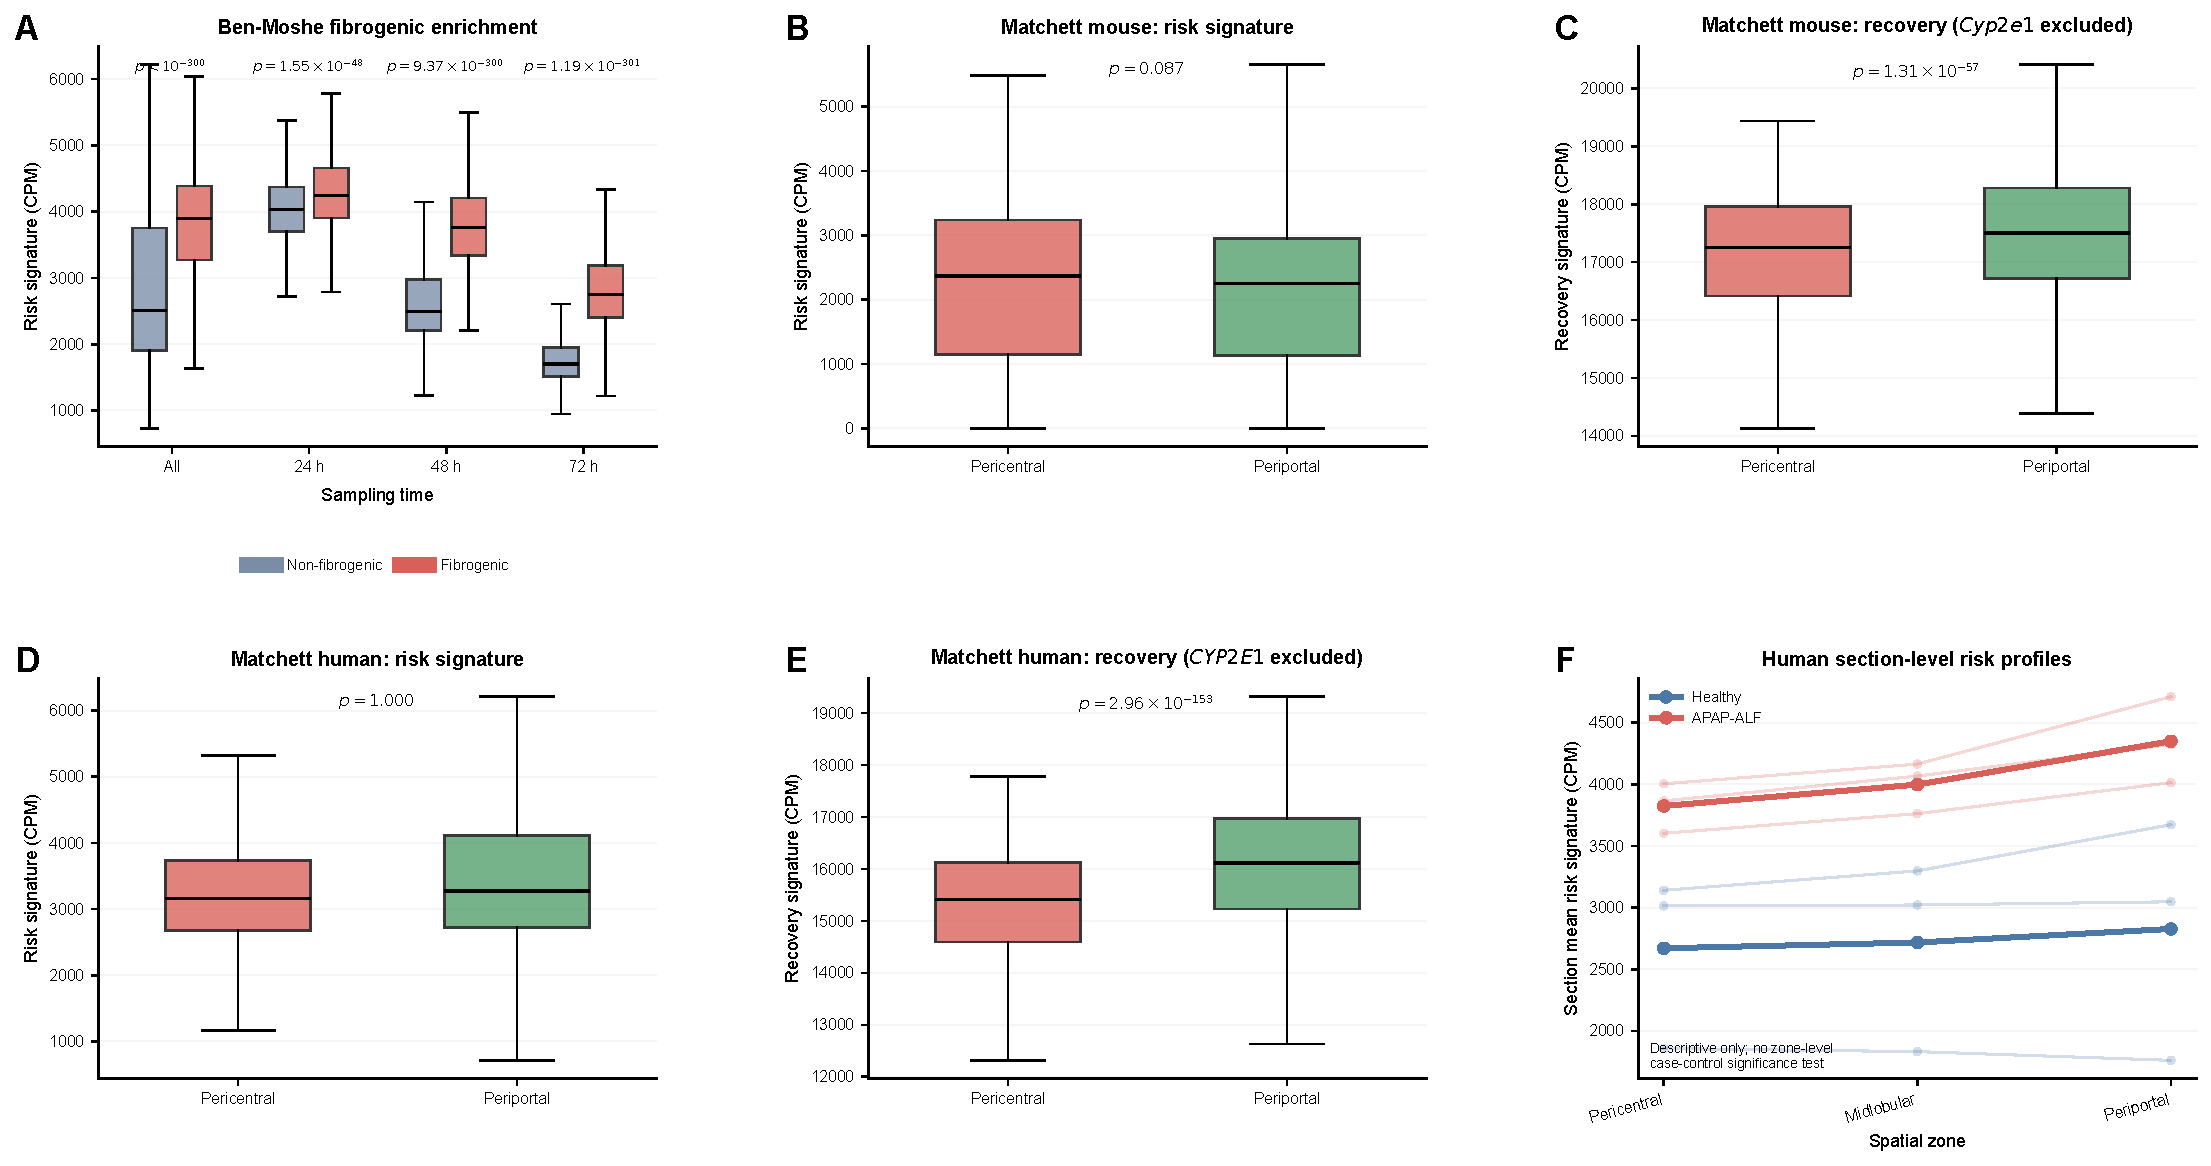
\includegraphics[width=0.64\textwidth,trim={356.000bp 0.000bp 354.415bp 285.000bp},clip]{figures/figure_S4.pdf}
\par\vspace{12pt}
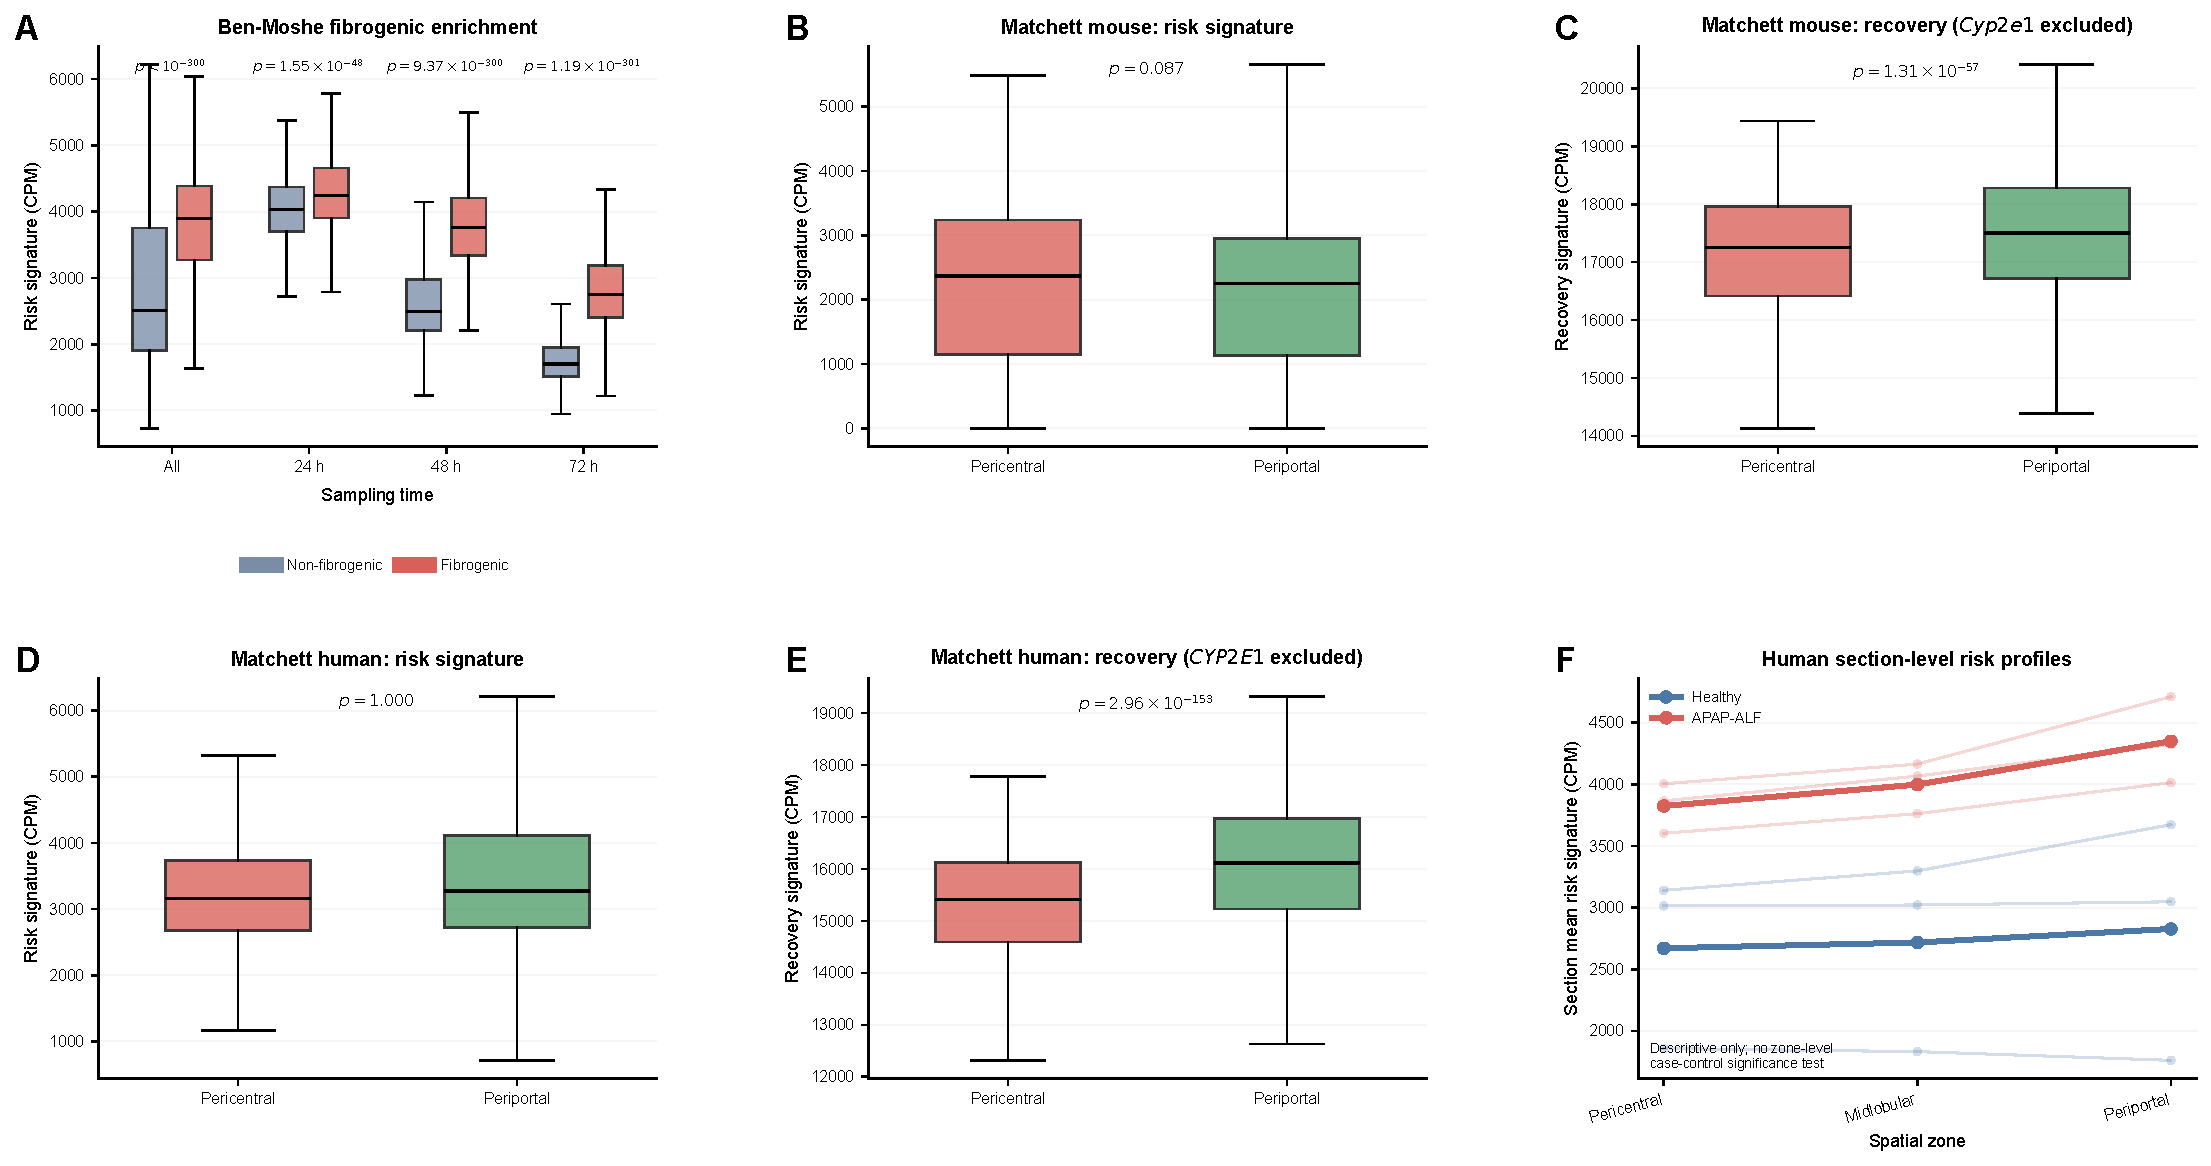
\includegraphics[width=0.64\textwidth,trim={708.000bp 0.000bp 0.000bp 285.000bp},clip]{figures/figure_S4.pdf}
\caption{\textbf{\FigSFourTitle{} (continued)} \textbf{(E)} \FigSFourE{} \textbf{(F)} \FigSFourF{} \FigSFourNotes{}}
\end{figure}

\clearpage
\begin{figure}[H]
\centering
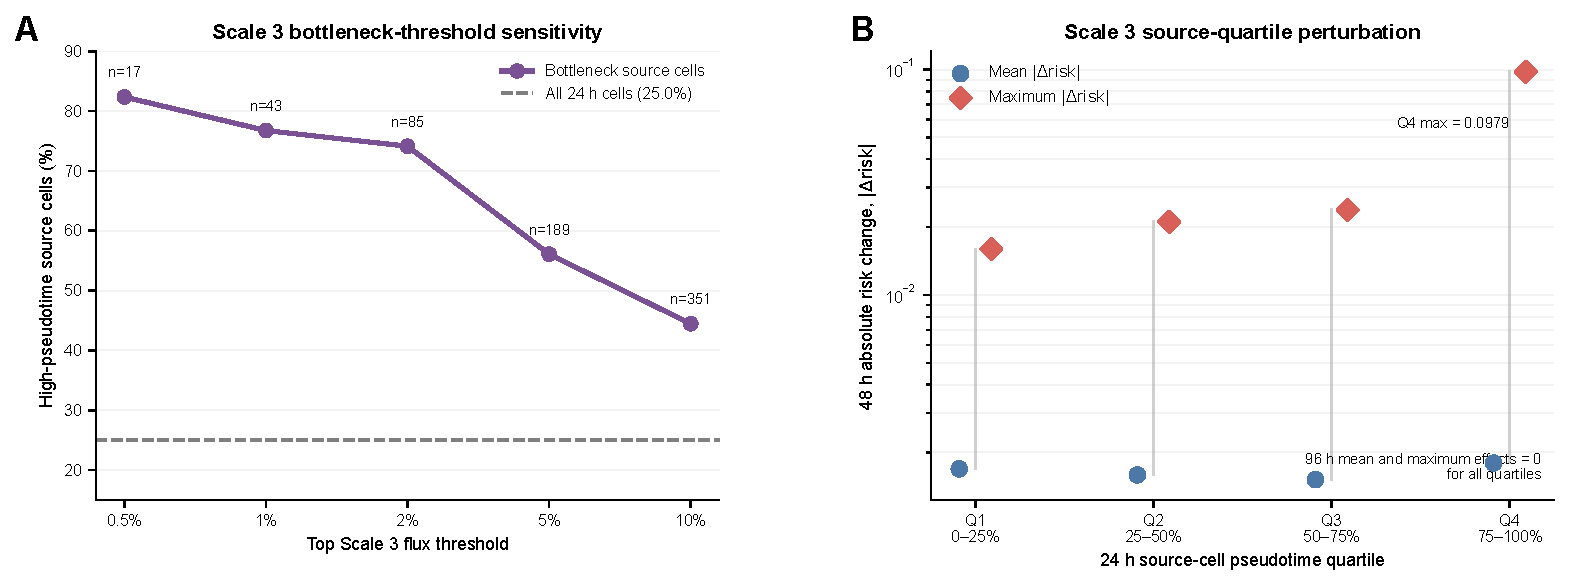
\includegraphics[width=0.68\textwidth,trim={0.000bp 0.000bp 377.120bp 0.000bp},clip]{figures/figure_S5.pdf}
\par\vspace{12pt}
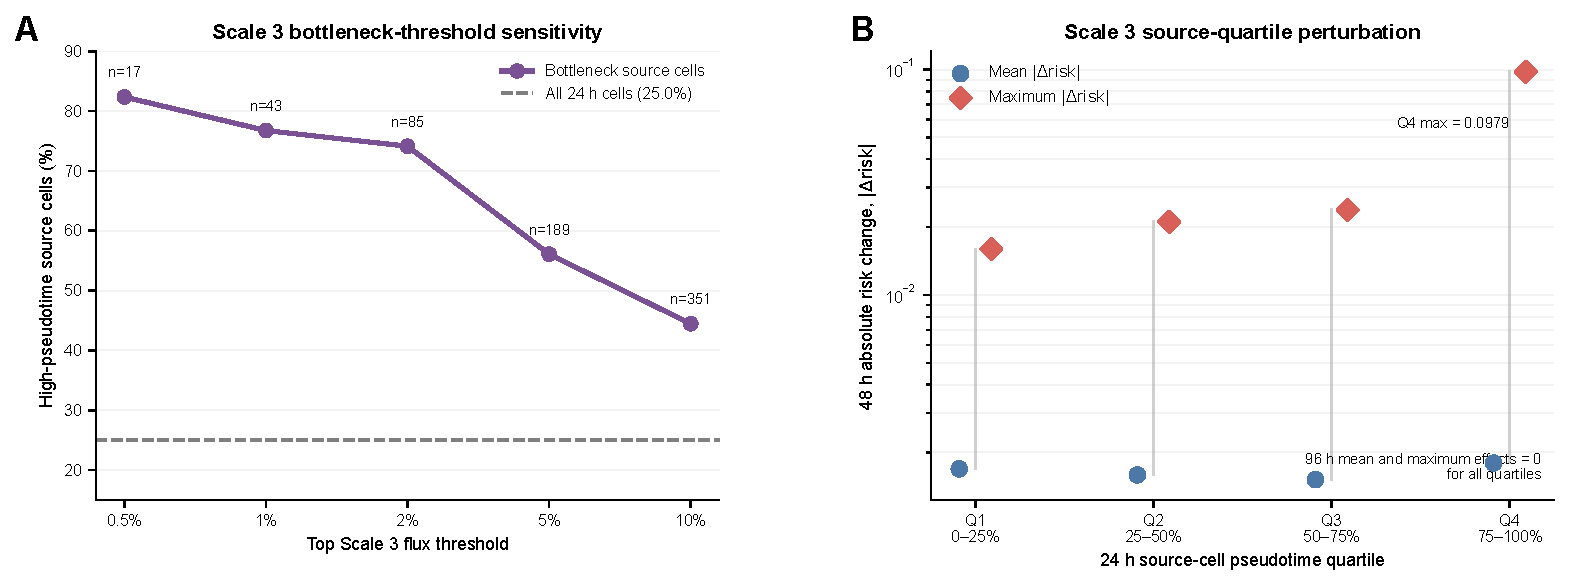
\includegraphics[width=0.68\textwidth,trim={377.000bp 0.000bp 0.000bp 0.000bp},clip]{figures/figure_S5.pdf}
\caption{\textbf{\FigSFiveTitle{}} \textbf{(A)} \FigSFiveA{} \textbf{(B)} \FigSFiveB{} \FigSFiveNotes{}}
\label{fig:S5}
\end{figure}
